\documentclass{article}
\usepackage[utf8]{inputenc}
\usepackage[T2A]{fontenc}
\usepackage[english,russian]{babel}
\usepackage[left=1.5cm,right=1.5cm,top=2cm,bottom=2cm]{geometry}
\usepackage{hyperref}
\usepackage{enumitem}
\usepackage{graphicx} %библиотека для графики и картинок
\DeclareGraphicsExtensions{.pdf,.png,.jpg}
\usepackage{listings}


\begin{document}
% НАЧАЛО ТИТУЛЬНОГО ЛИСТА
\begin{center}
    \Large
    Федеральное государственное автономное \\
    образовательное учреждение высшего образования \\ 
    «Национальный исследовательский университет ИТМО»\\
    \vspace{0.5cm}
    \large
    
    \vspace{1cm}
    \Large
    \textbf{По дисциплине «Информационная безопасность»} \\
        Лабораторная работа №4\\
        Аудит безопасности веб-приложения
    \large
    \vspace{8cm}

    \begin{minipage}{.33\textwidth}
    \end{minipage}
    \hfill
    \begin{minipage}{.4\textwidth}
    
        \textbf{Студент}: \vspace{.1cm} \\
        \ Дениченко Александр Олегович P3412\\
        \textbf{Практик}:  \\
        \ Маркина Татьяна Анатольевна
    \end{minipage}
    \vfill
Санкт-Петербург\\ 2025 г.
\end{center}
\pagestyle{empty}
% КОНЕЦ ТИТУЛЬНОГО ЛИСТА 
\newpage
\pagestyle{plain}

\section*{Цель}
Освоить методику комплексного анализа защищенности веб-приложения, сочетая
автоматизированное сканирование (DAST) и проактивное моделирование угроз (Threat Modeling).
Получить навыки документирования результатов аудита в виде профессионального отчета.

\section{Вводная часть}

Установил OWASP Juice Shop и запустил его локально.
\begin{center}
  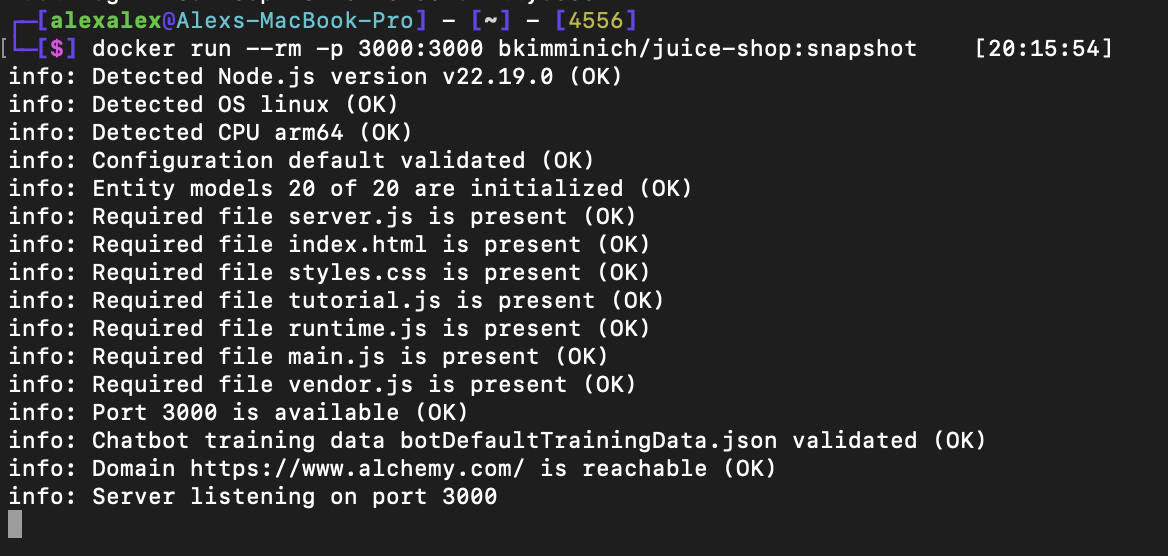
\includegraphics[width=.9\textwidth]{start}
\end{center}

\section{Первичное автосканирование}

Настройки выставил -- по стандарту использование традиционного паука + 
if modern -- использование firefox. Далее сделана атака.

Сделал Атаку, получил следующие результаты:
\begin{center}
  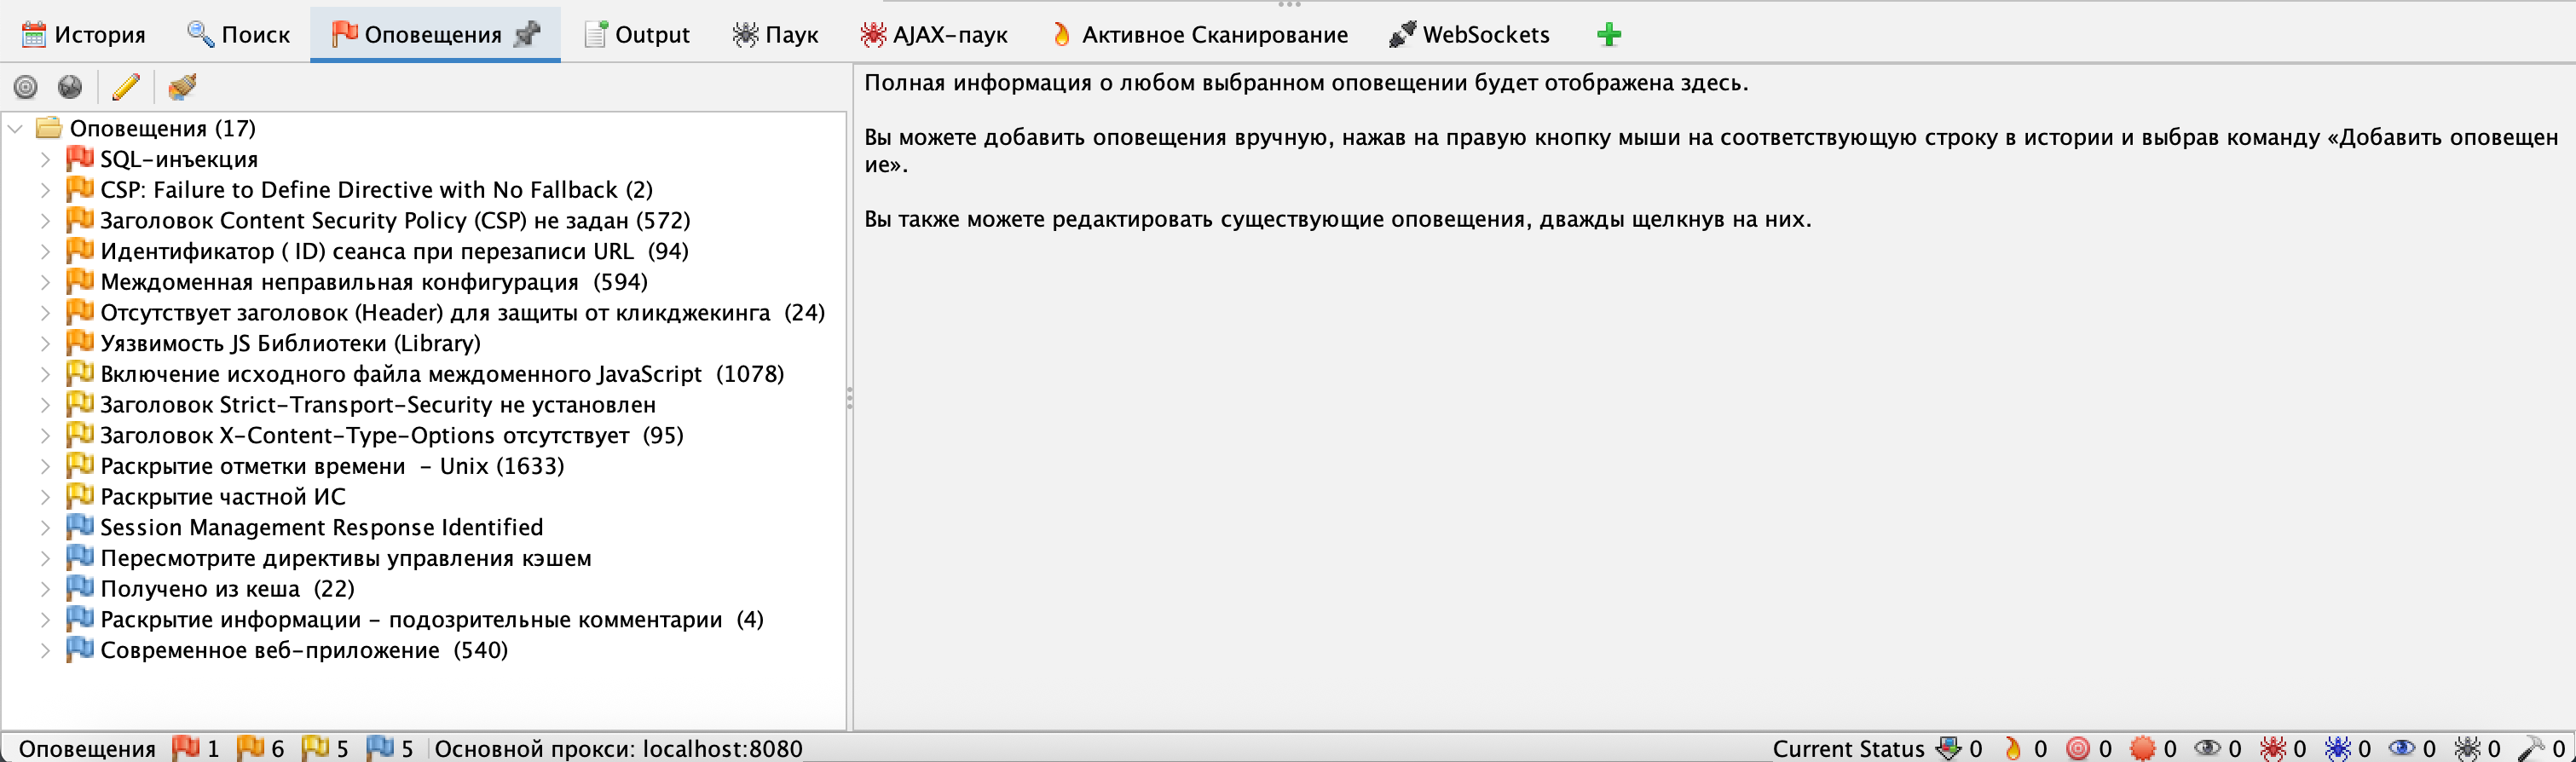
\includegraphics[width=.9\textwidth]{scan}
\end{center}

Было решено провести доп исследование через "Score
Board", чтобы получить больше уязвимостей уровня HIGH.

\begin{center}
  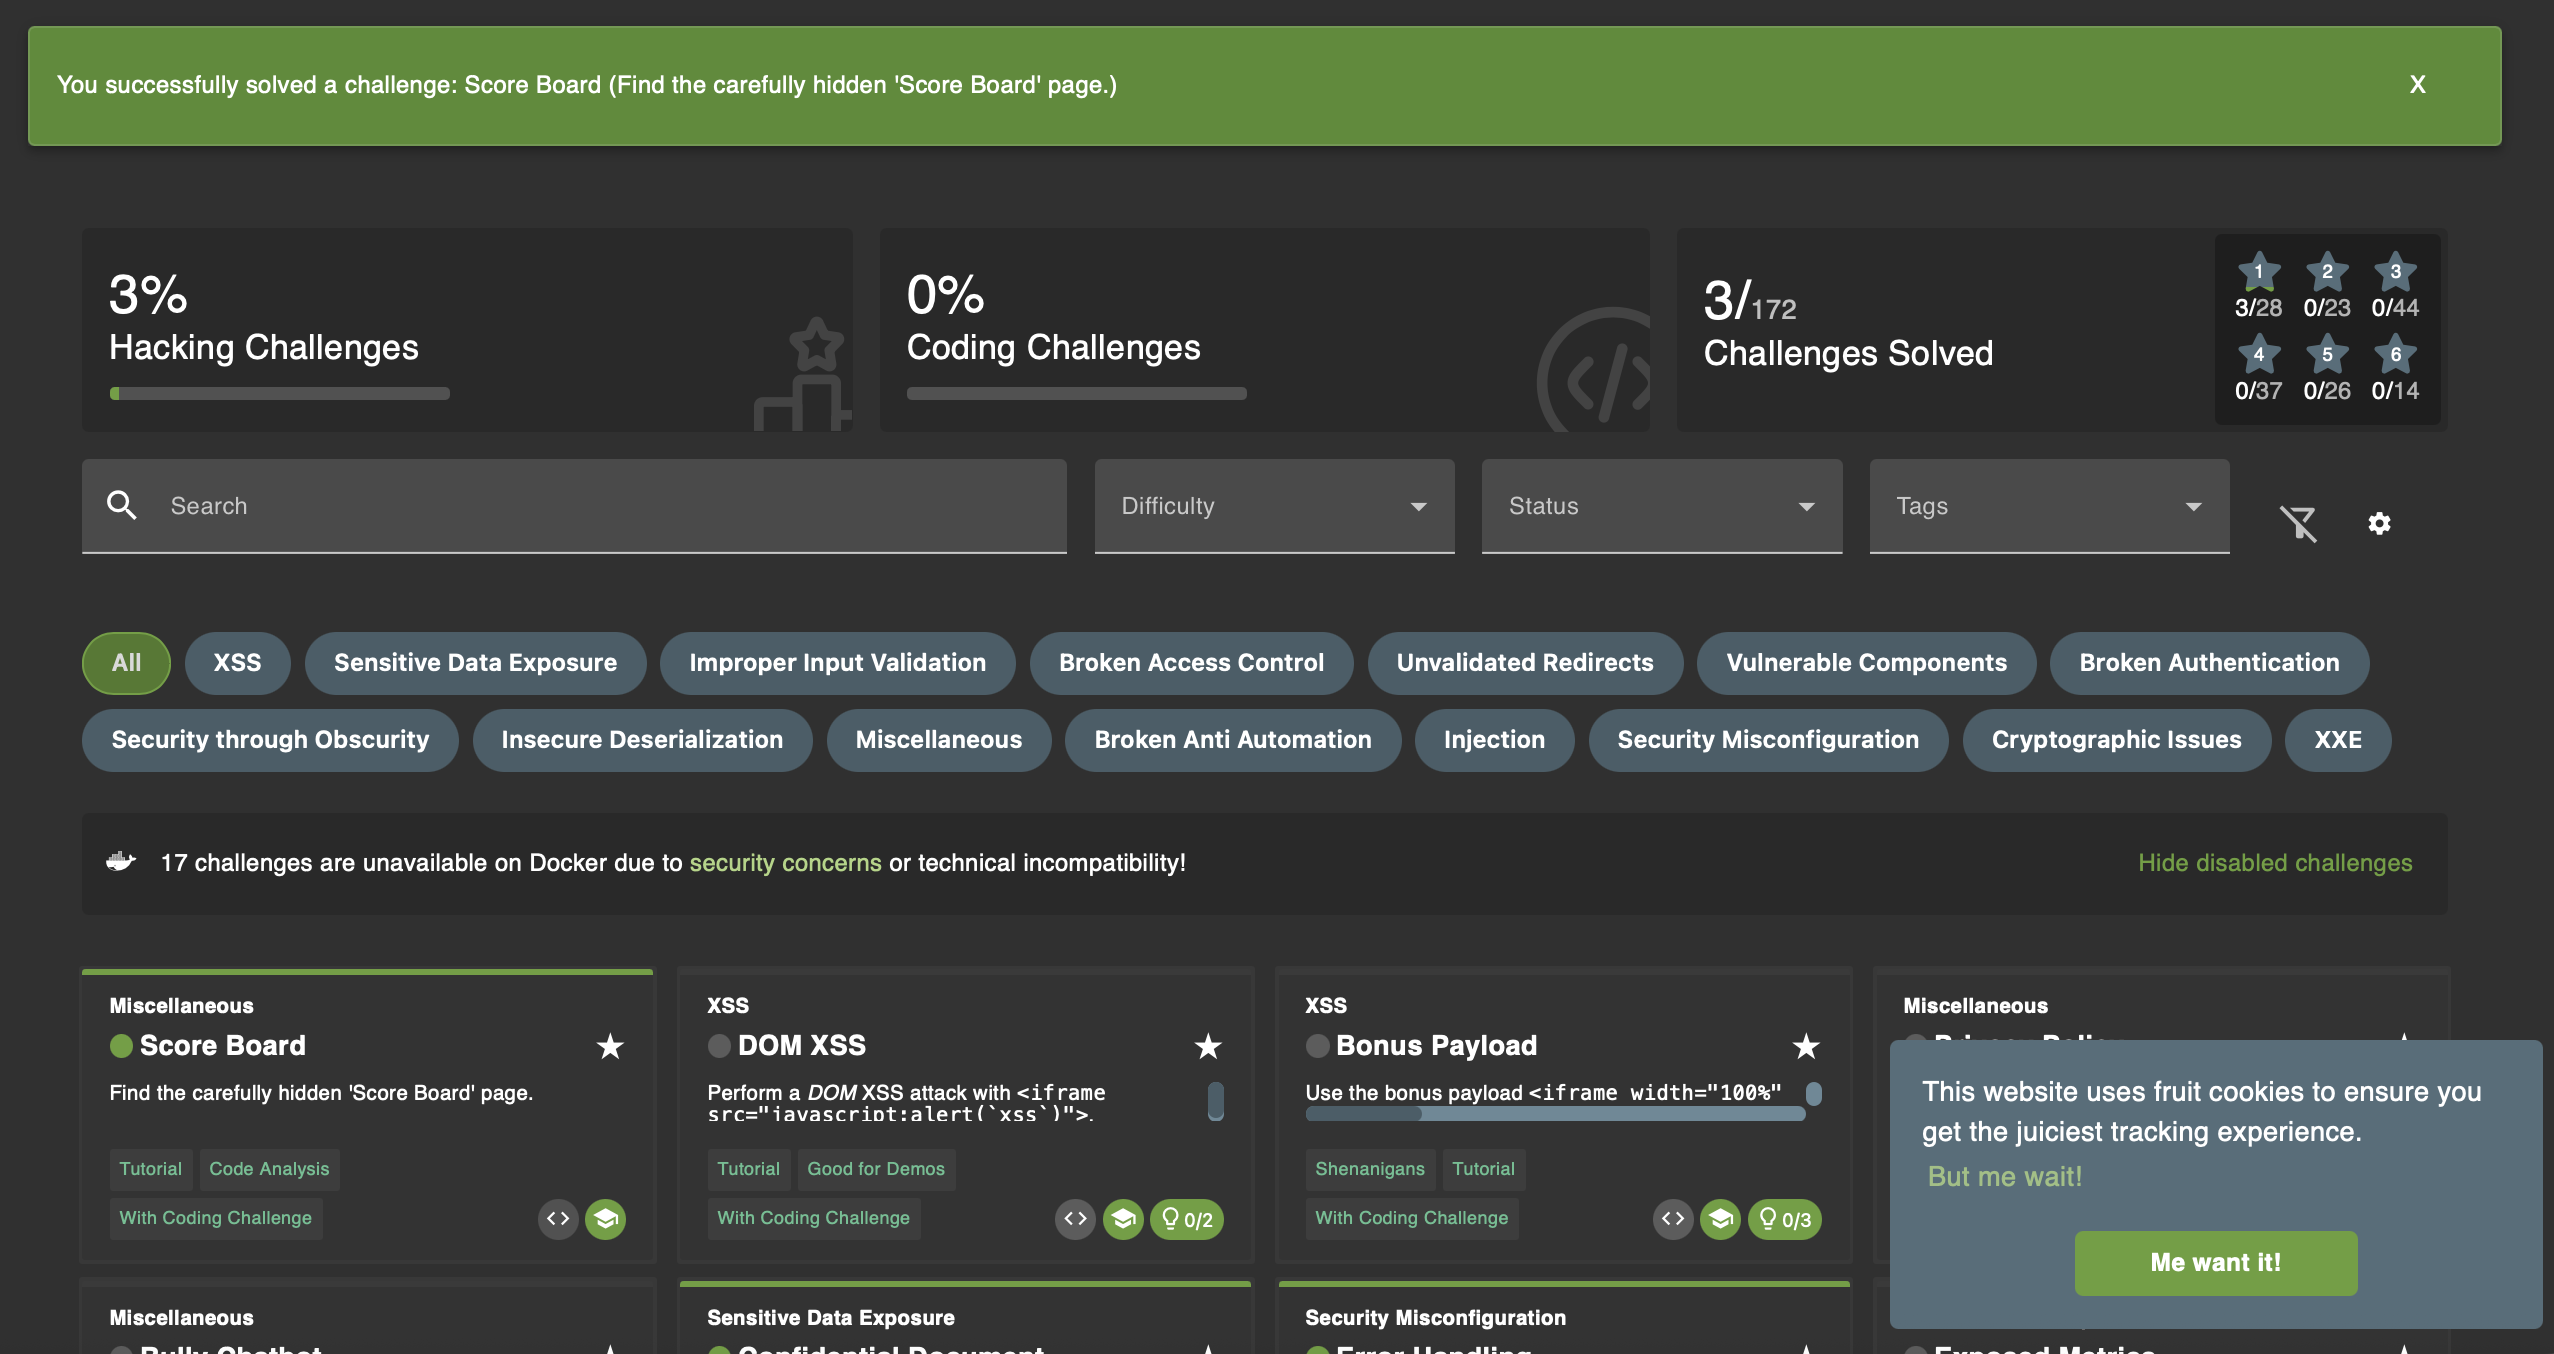
\includegraphics[width=.9\textwidth]{br}
\end{center}

\section{Нахождении и подтверждение уязвимостей}

\subsection{SQL Injection 1}
Попробуем залогиниться и ввести следующие данные:

\begin{center}
  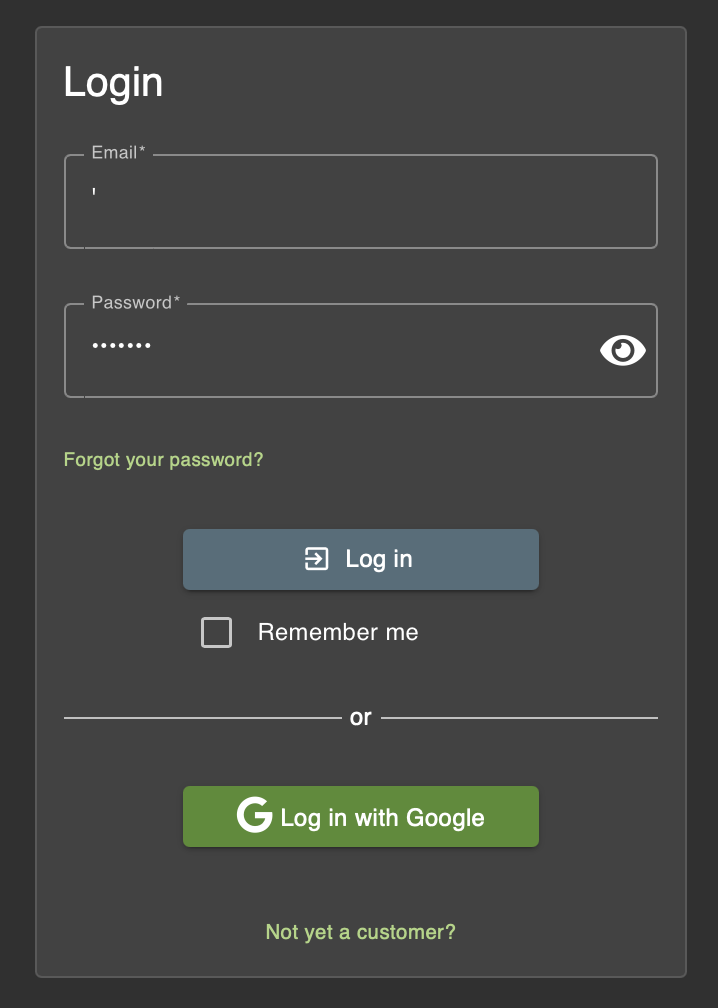
\includegraphics[width=.4\textwidth]{i1}
\end{center}

Как можно увидеть получилось провести SQL Injection так как символ из логина не заэкранировался. 
\begin{center}
  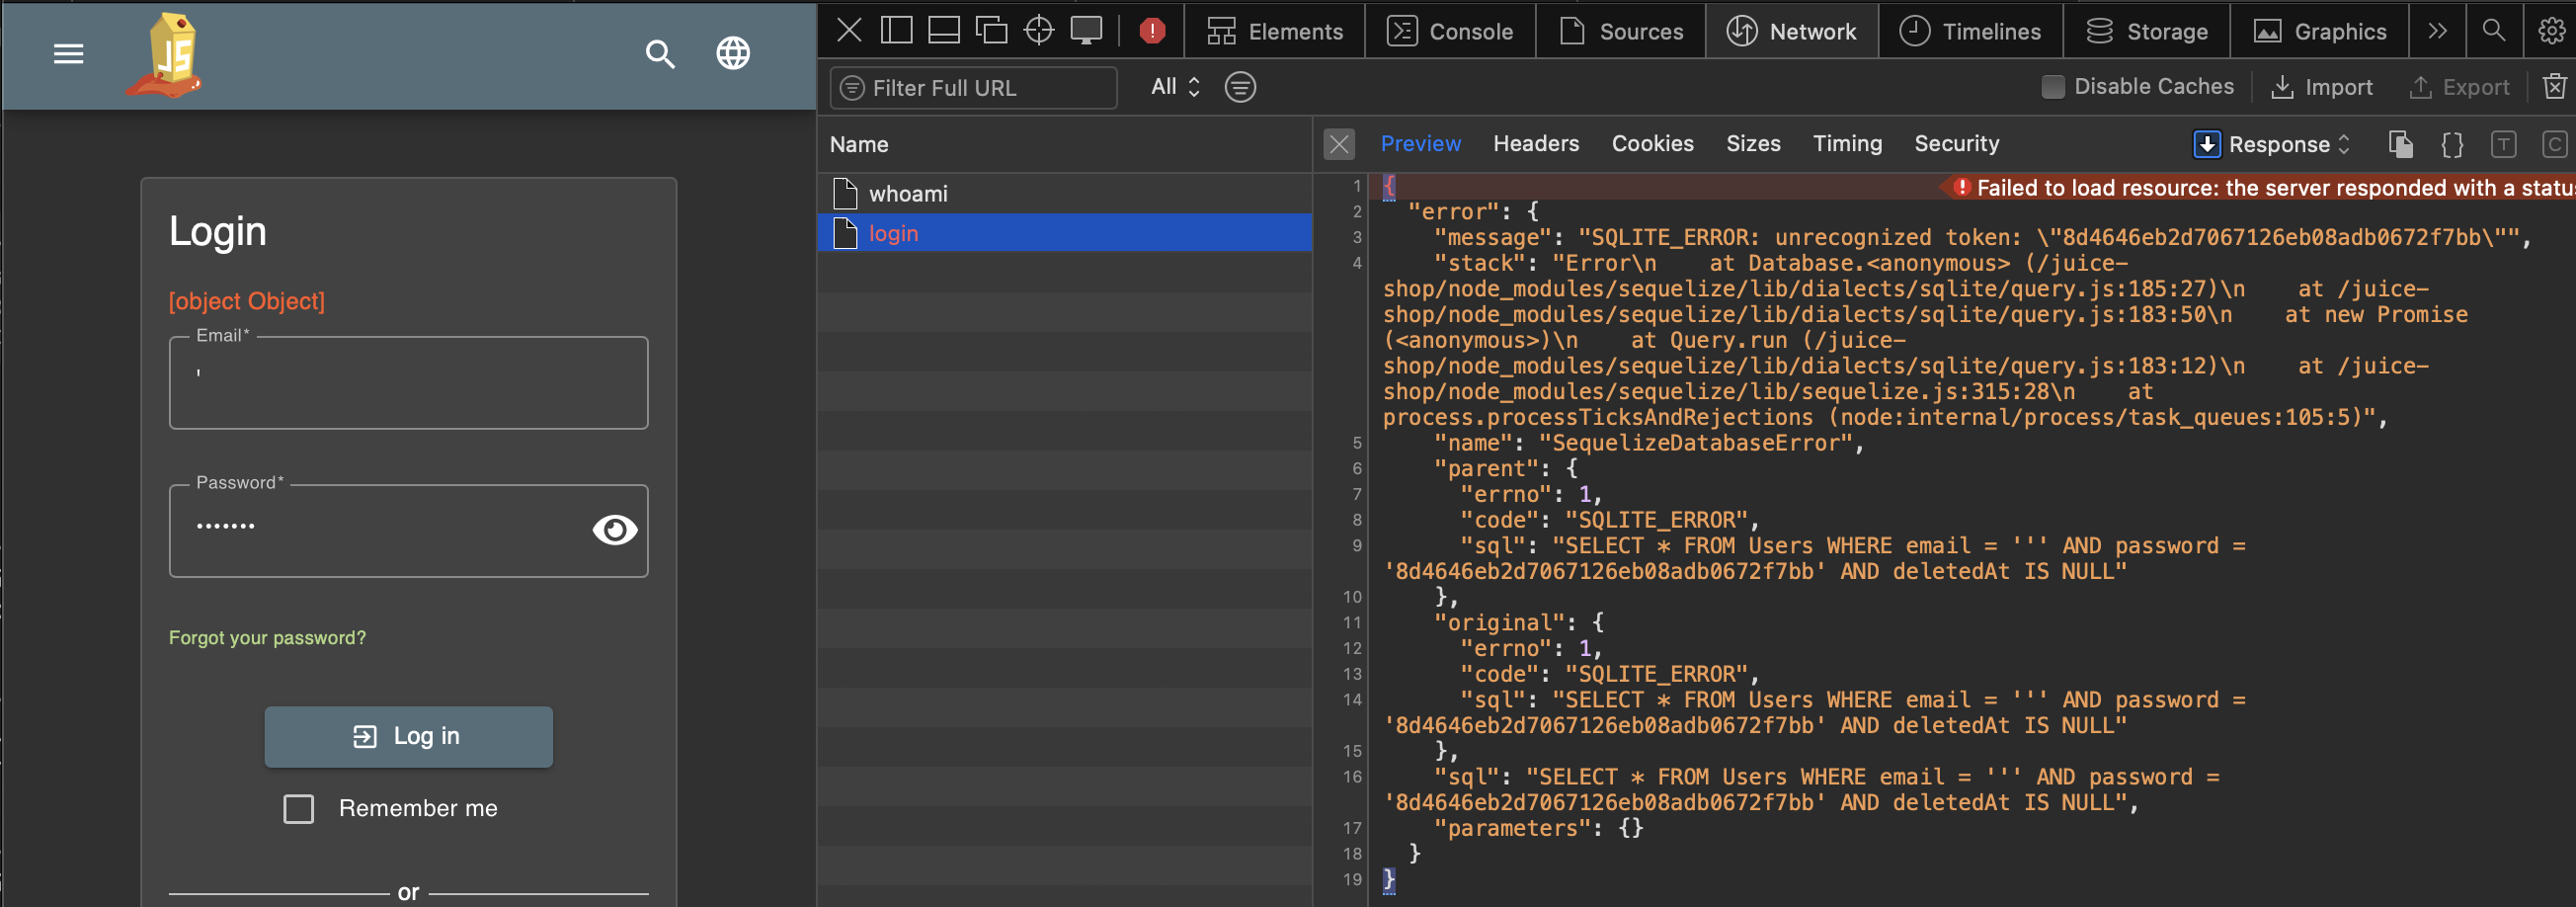
\includegraphics[width=.9\textwidth]{i11}
\end{center}

Зайдём под админом
\begin{center}
  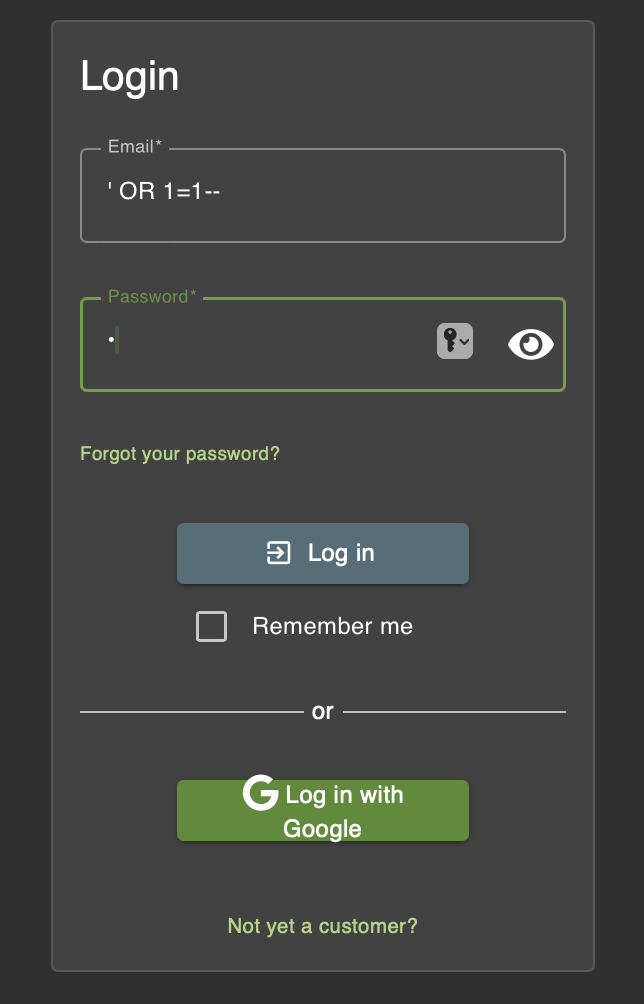
\includegraphics[width=.4\textwidth]{i111}
\end{center}
Выполнится следующий запрос:

\begin{lstlisting}
  SELECT * FROM Users WHERE email = '' OR 1=1-- ' AND password = '...';
\end{lstlisting}
Успешно
\begin{center}
  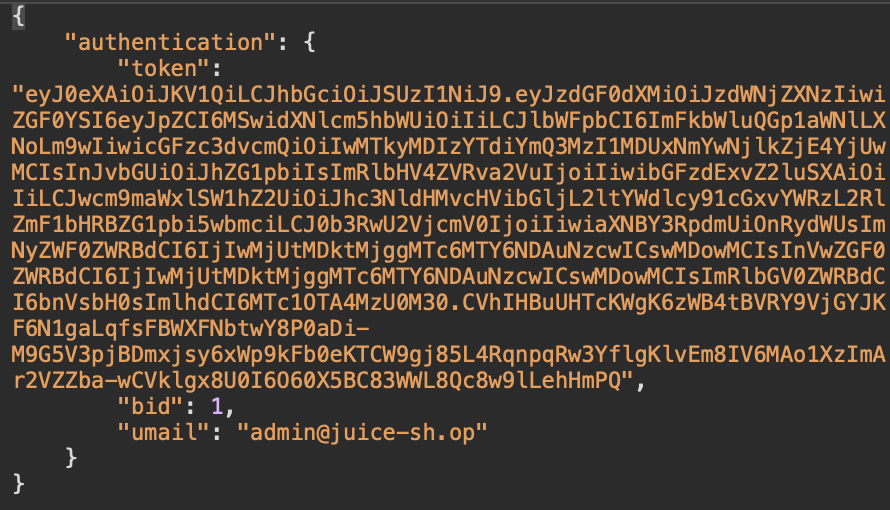
\includegraphics[width=.9\textwidth]{i1111}
\end{center}

\subsection{XSS}

Попробуем ввести следующие данные поле поиска:

\begin{lstlisting}
  <iframe src="javascript:alert(`xss`)">
\end{lstlisting}

Наш код встроился в страницу.
\begin{center}
  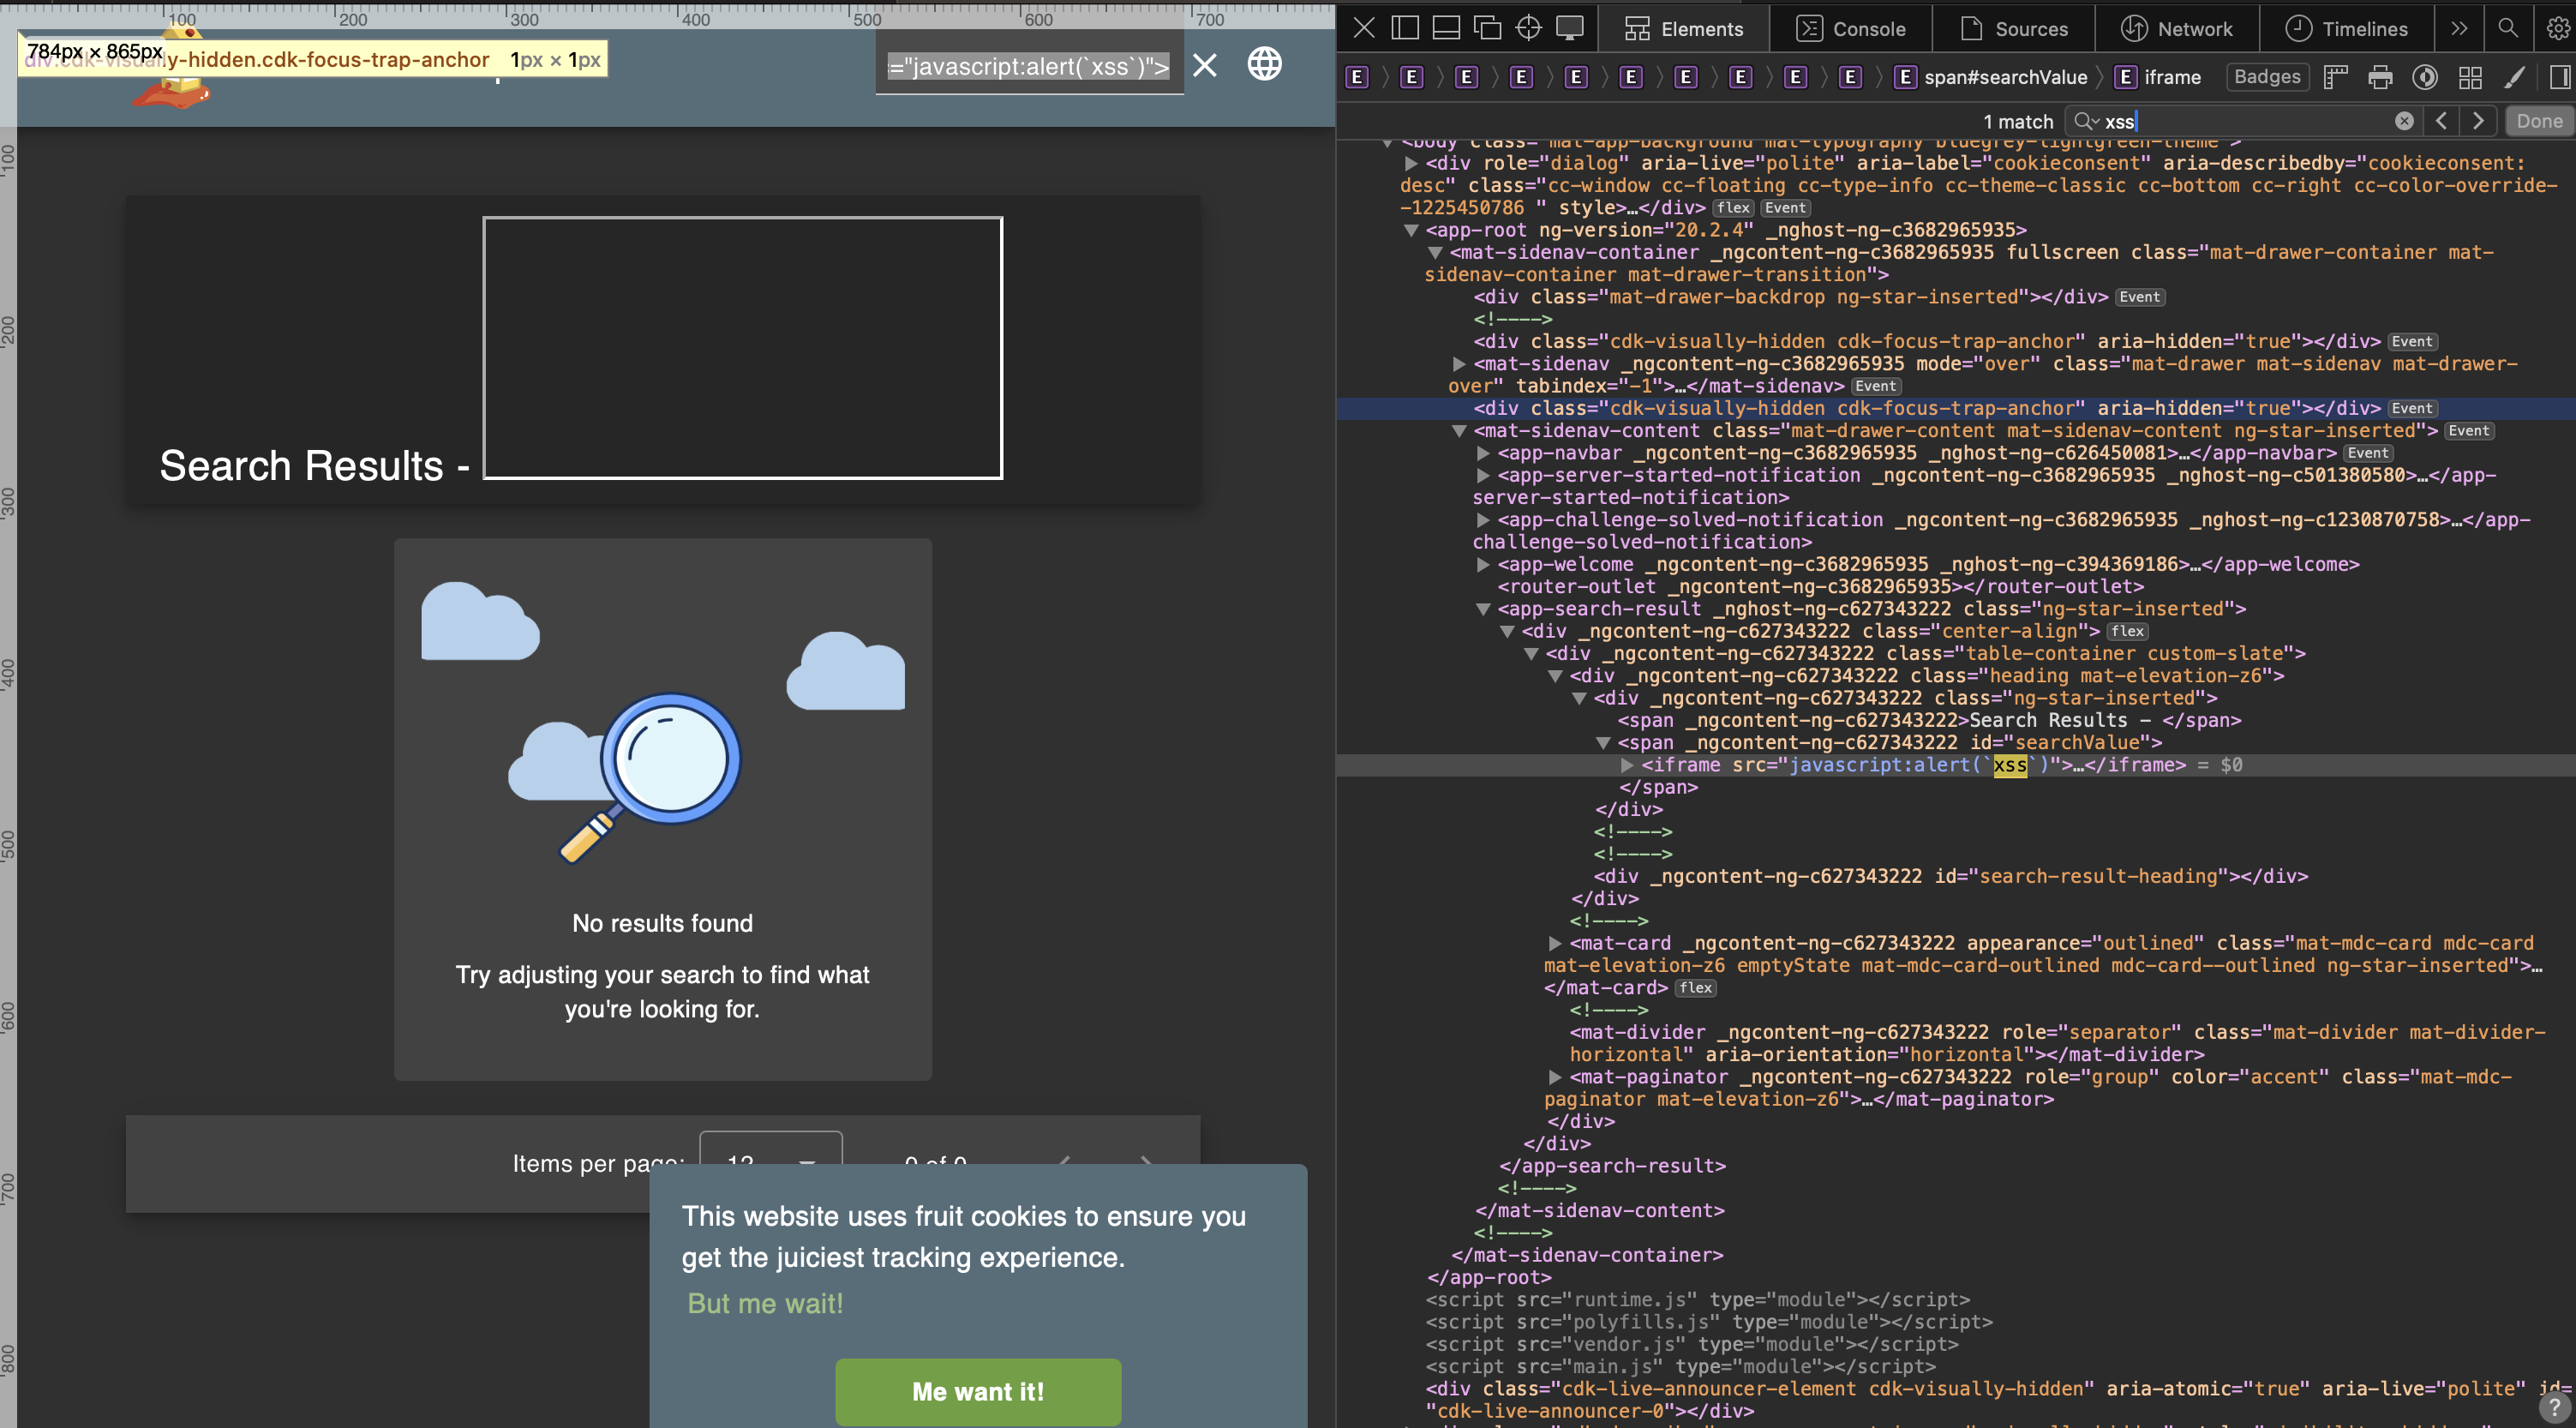
\includegraphics[width=.9\textwidth]{x1}
\end{center}

При открытии страницы теперь у всех пользователей будет выполняться XSS этого вида.

\begin{center}
  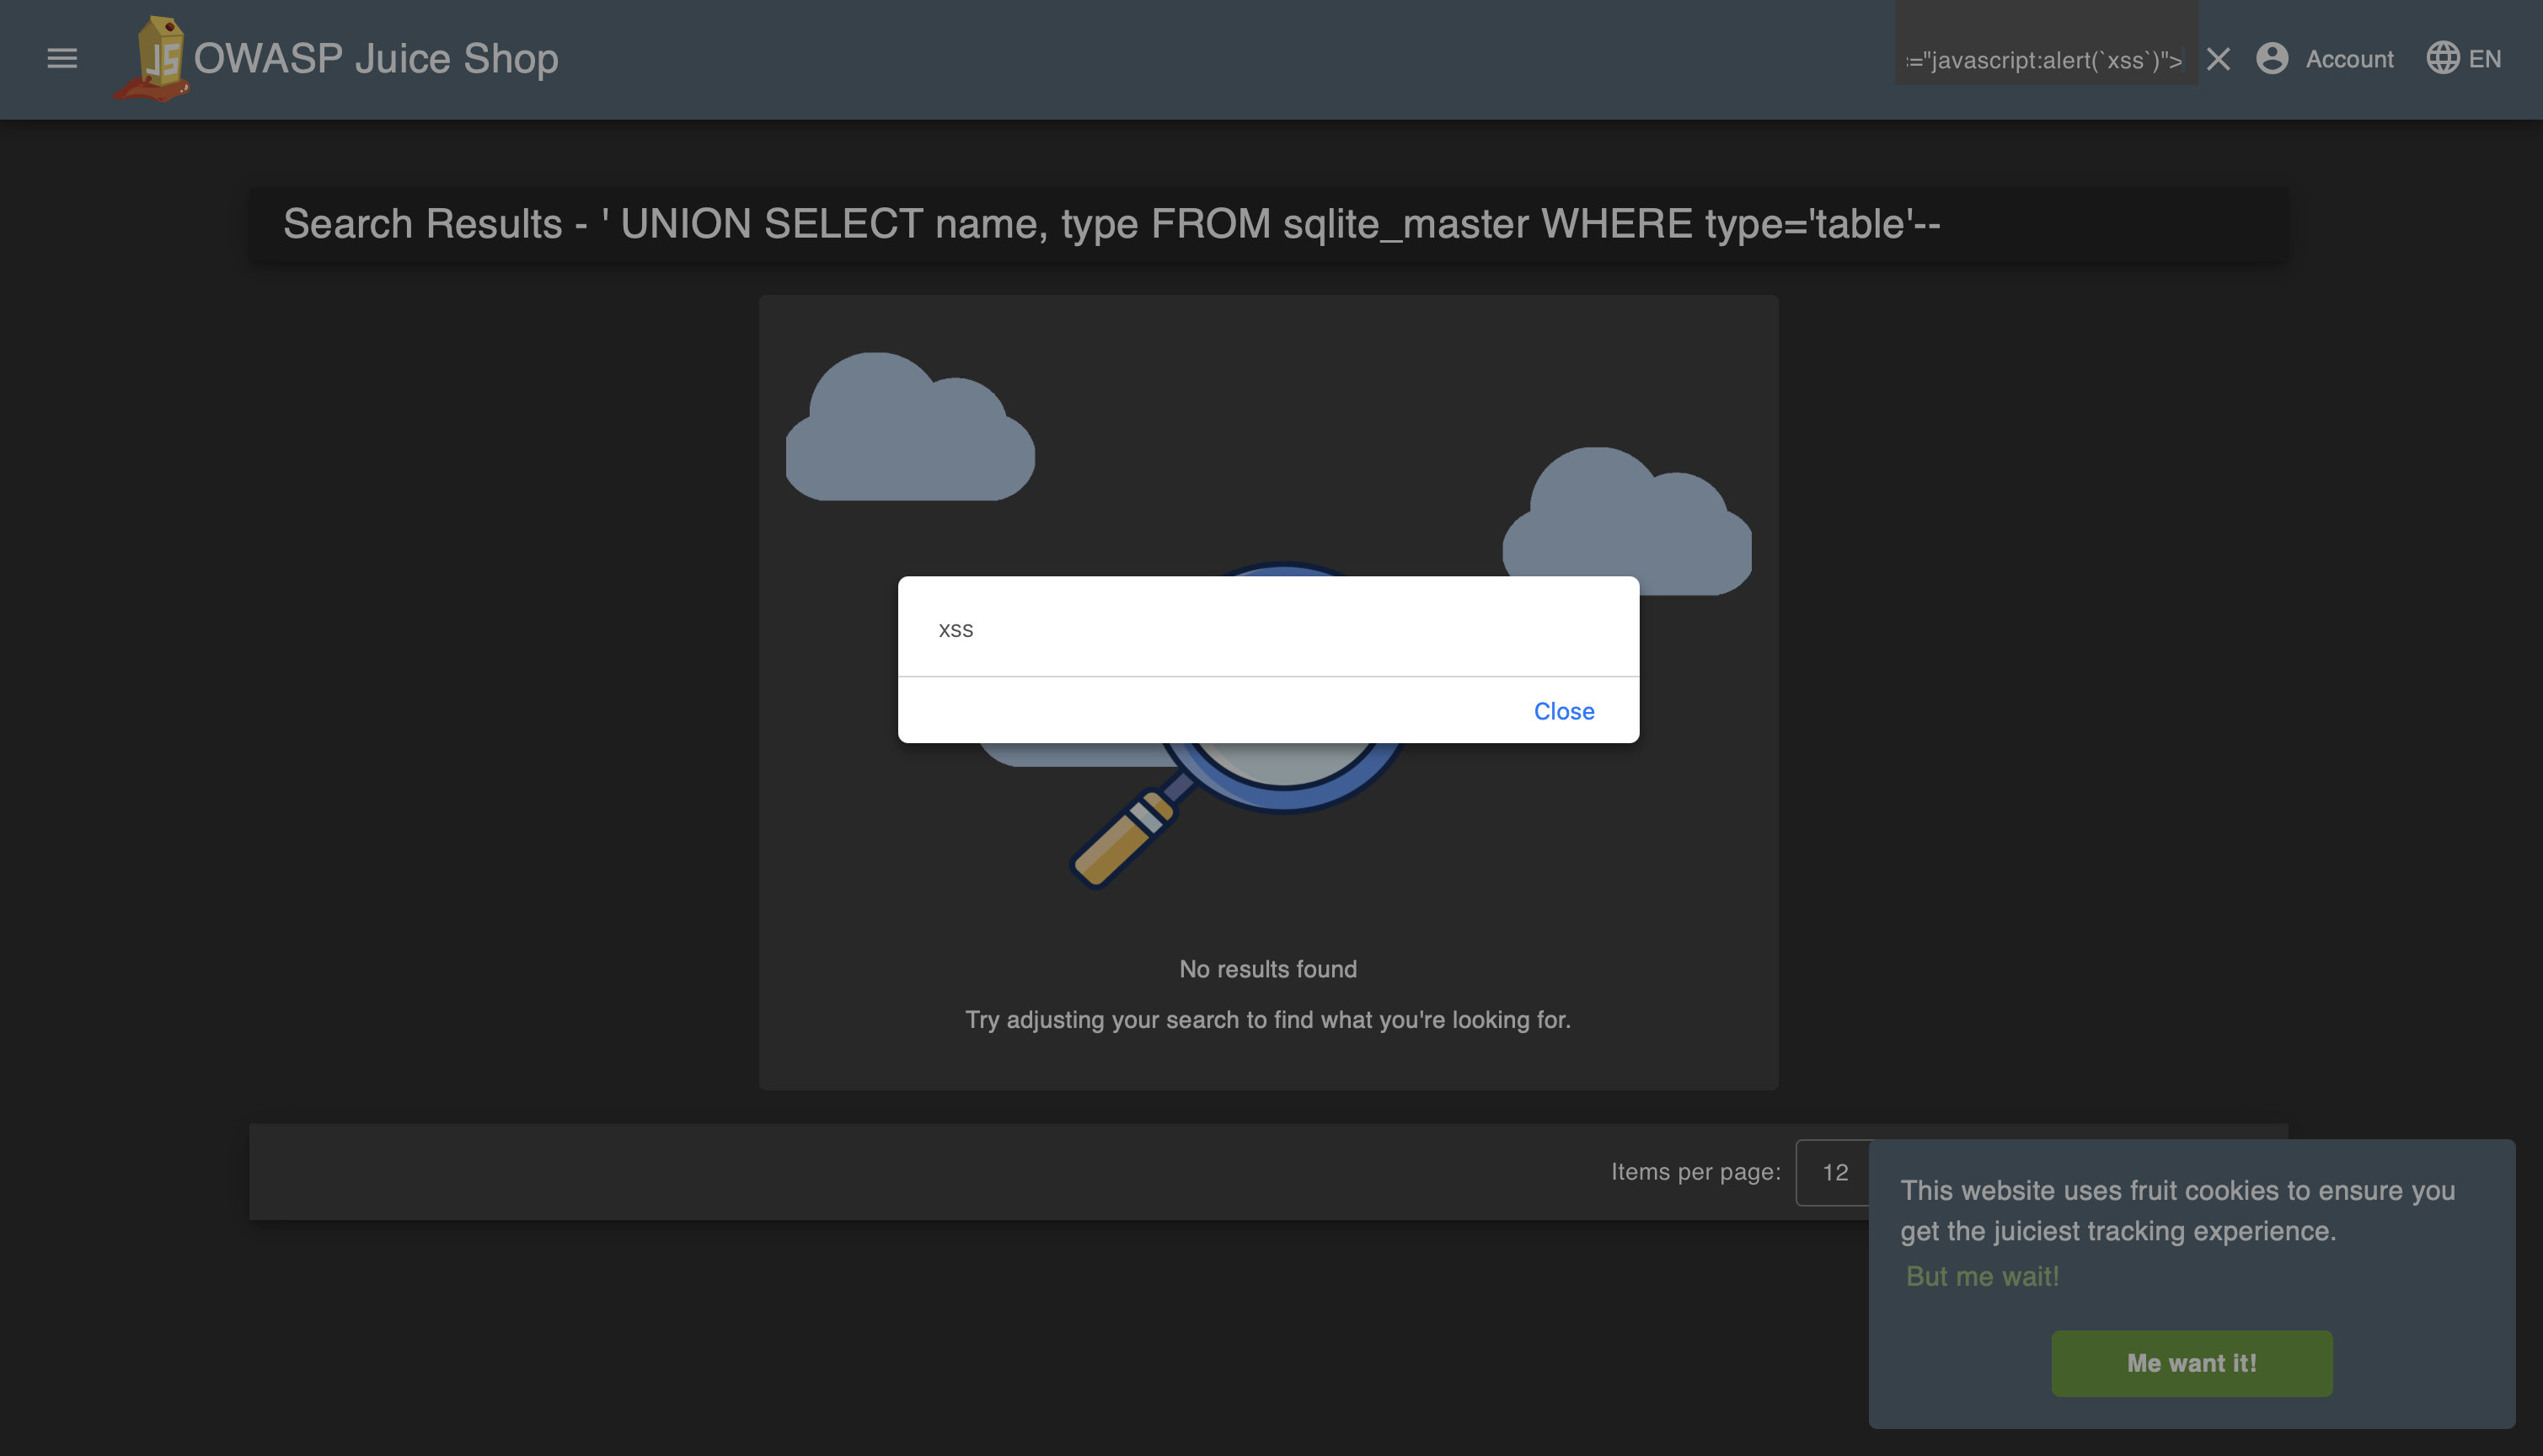
\includegraphics[width=.9\textwidth]{x11}
\end{center}


\subsection{Sensitive Data Exposure. Exposed credentials}

Попробуем получить пароль и логин из исходного кода. Перейдём во вкладку "Sources" в dev tools. И сделаем поиск по строке "username".

\begin{center}
  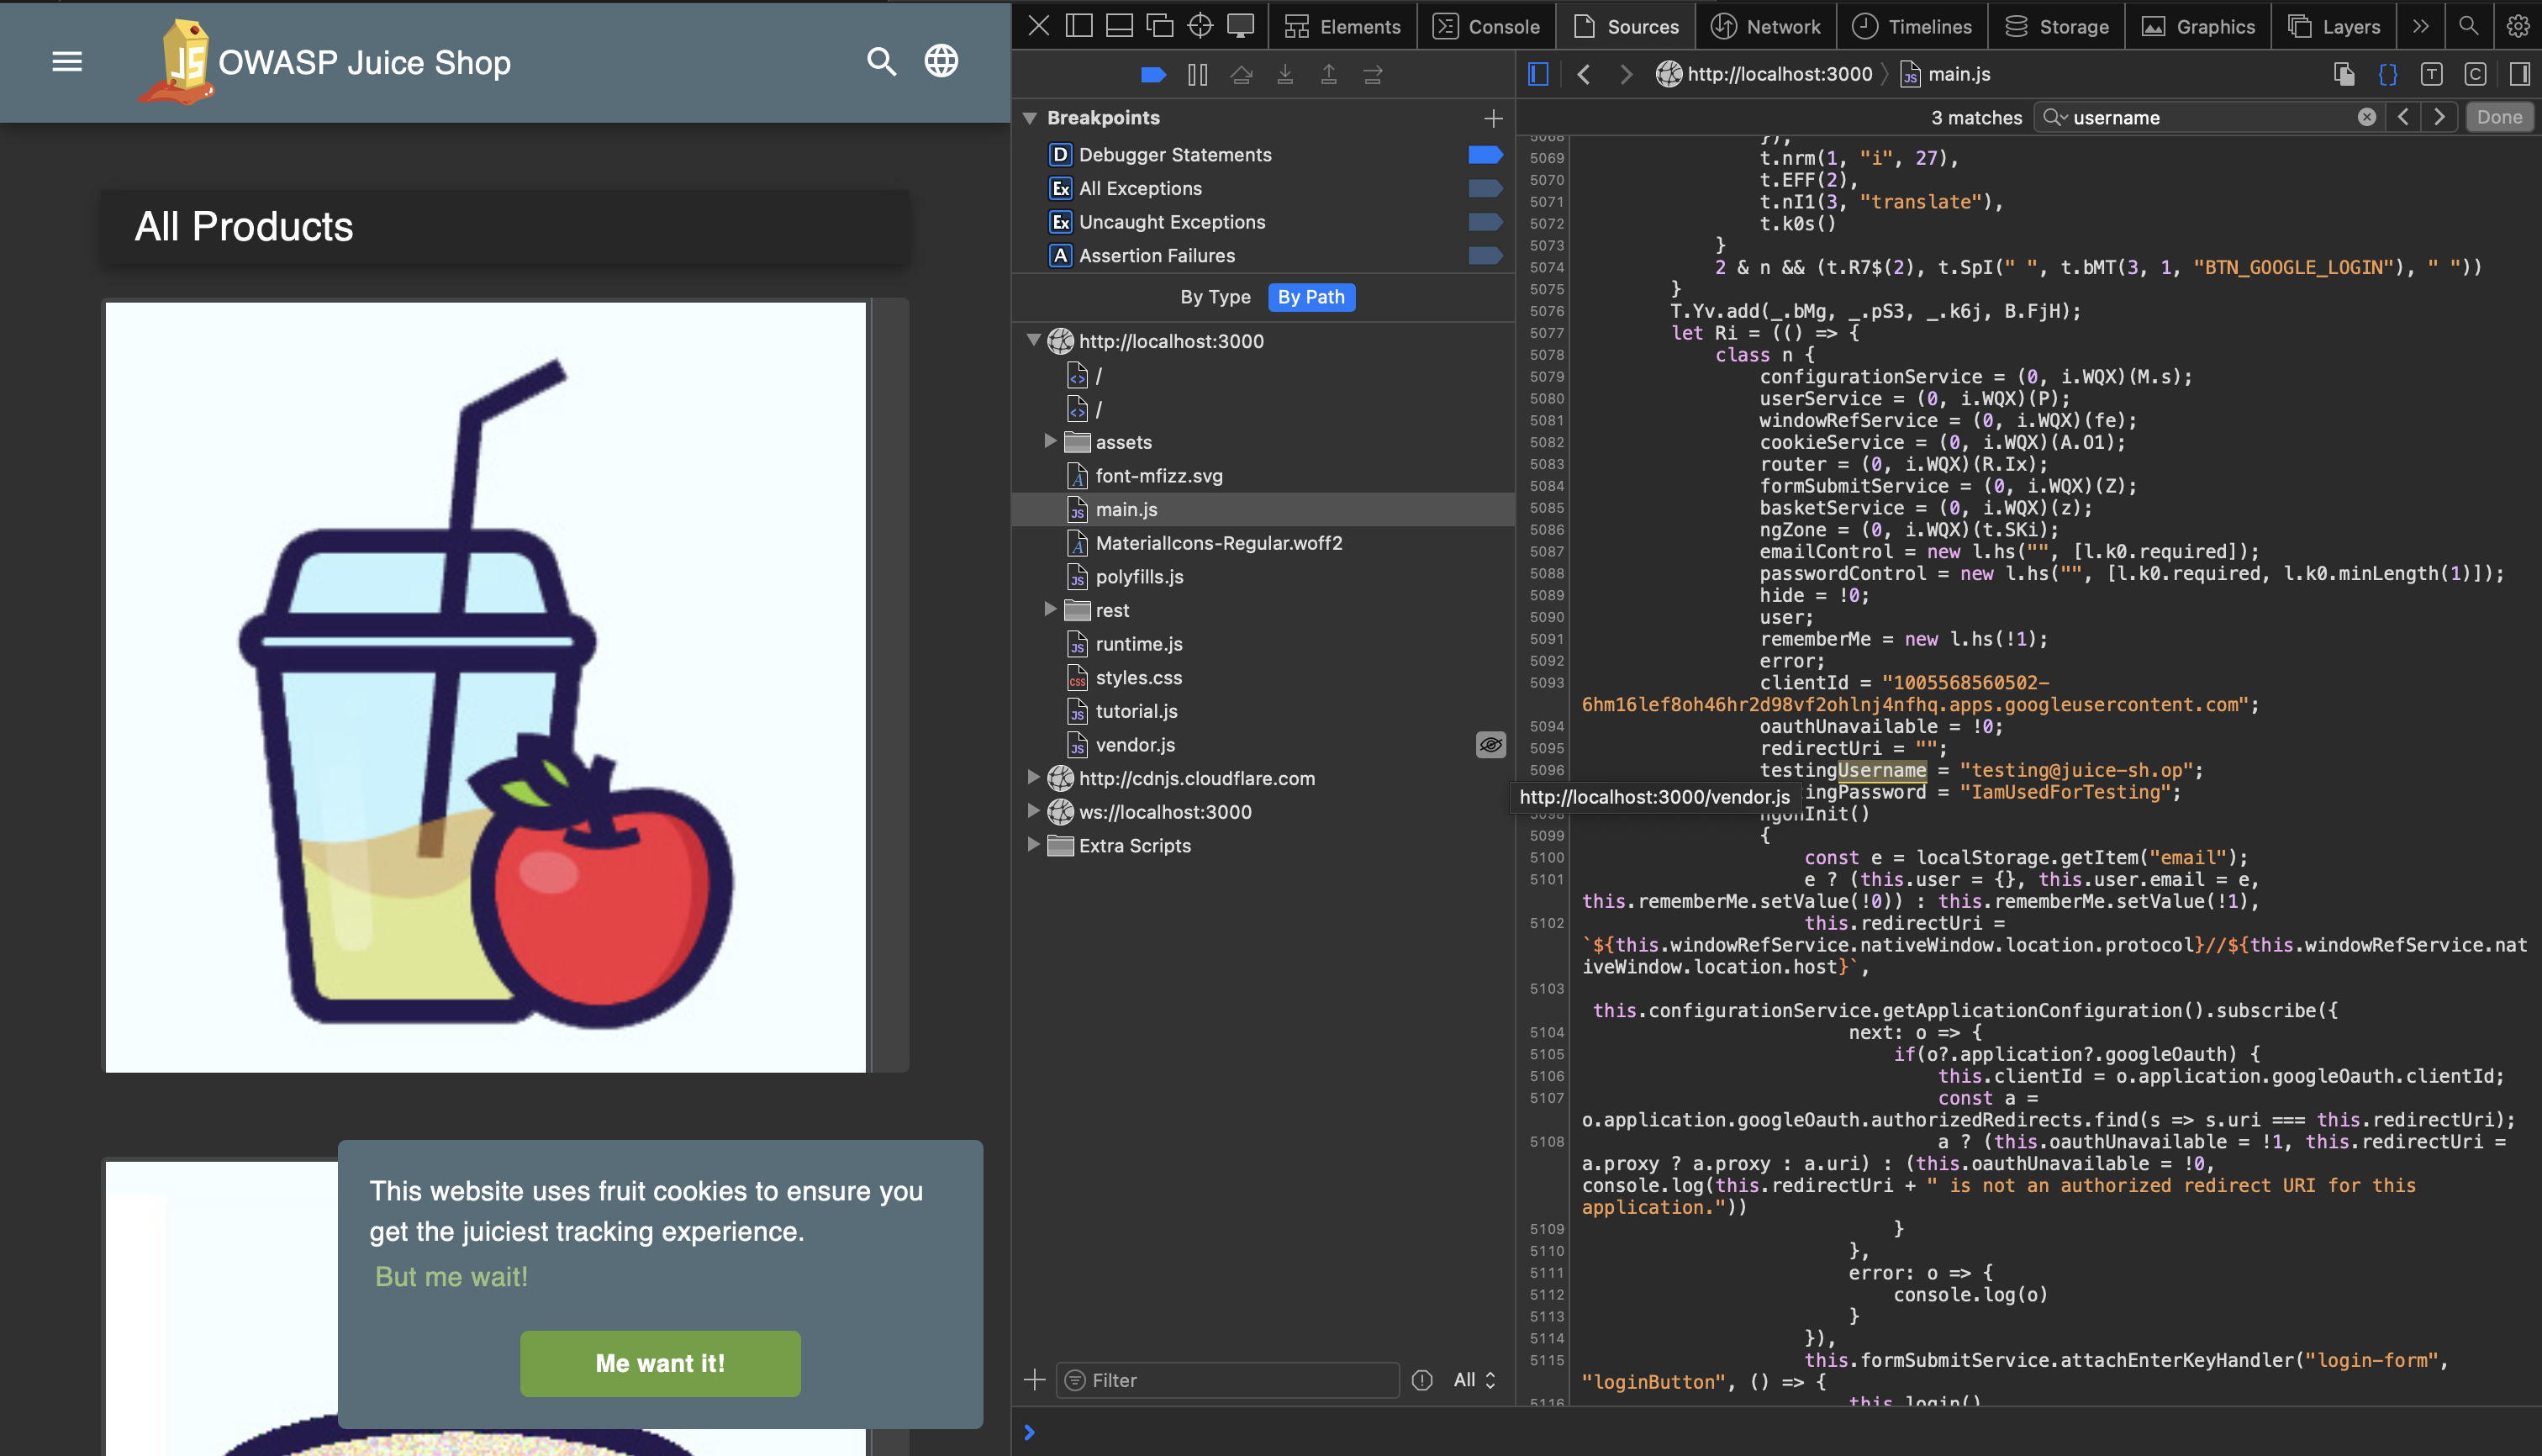
\includegraphics[width=.9\textwidth]{e1}
\end{center}

Мы видим, что пароль и логин находятся в файле "main.js" и его легко использовать для входа в систему.
Проверим вход.

\begin{center}
  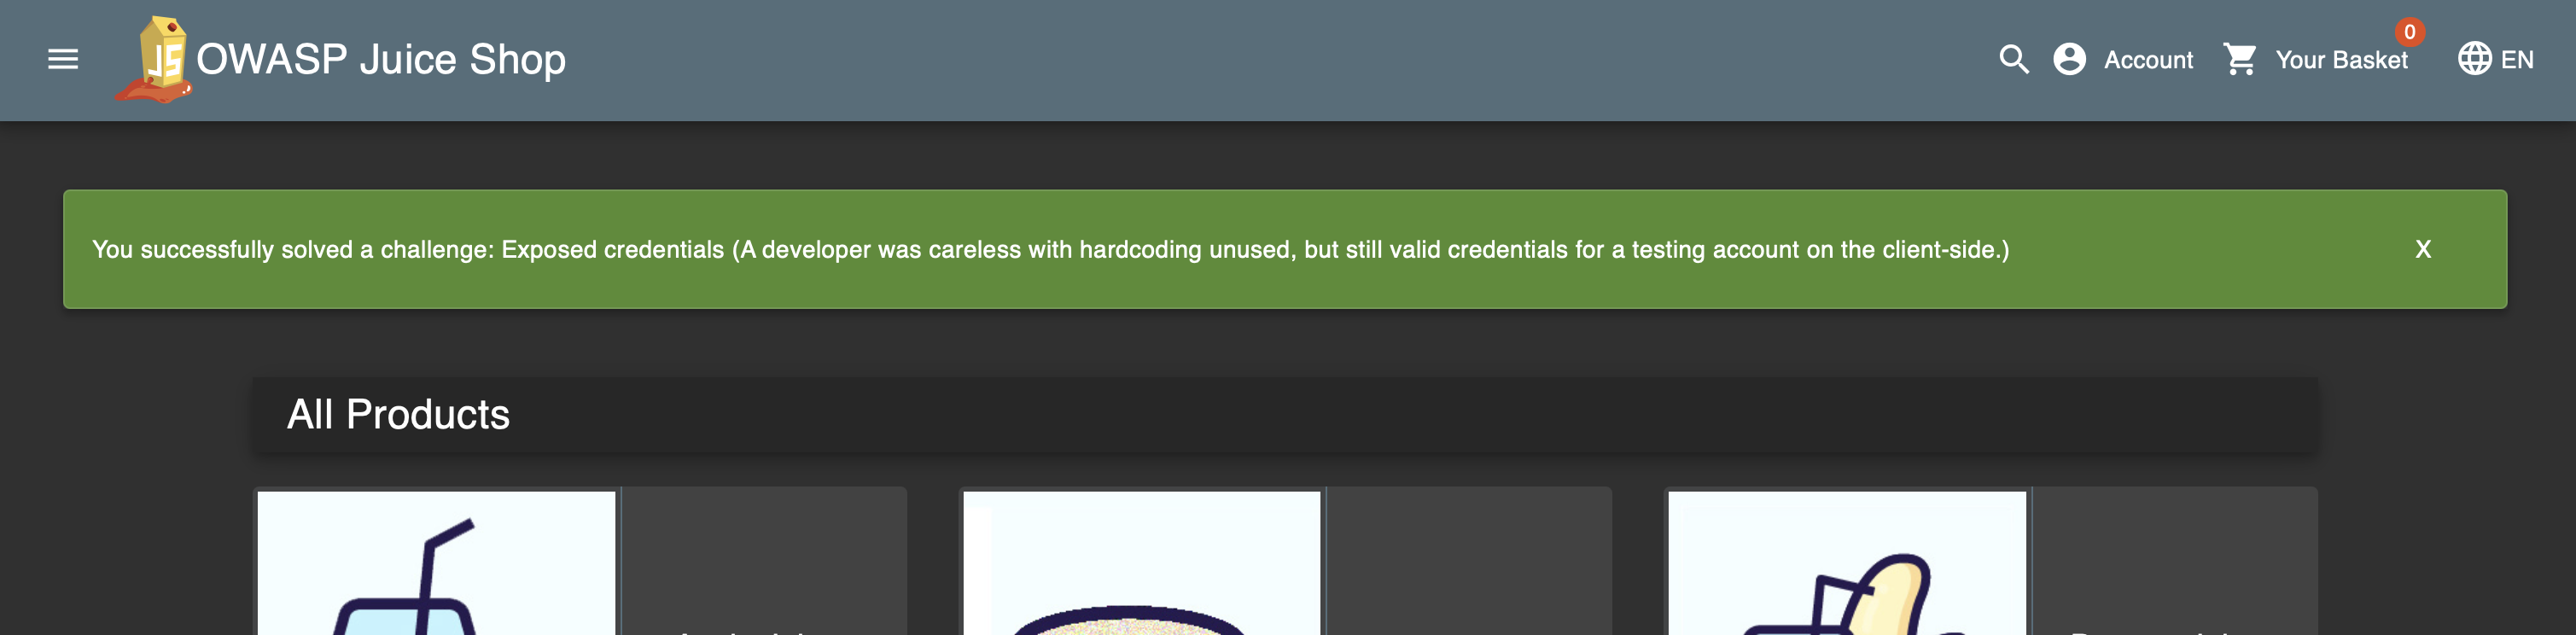
\includegraphics[width=.9\textwidth]{e11}
\end{center}

Всё работает.

\subsection{Broken Access Control}

Попробуем получить доступ к чужой корзине.
\begin{center}
  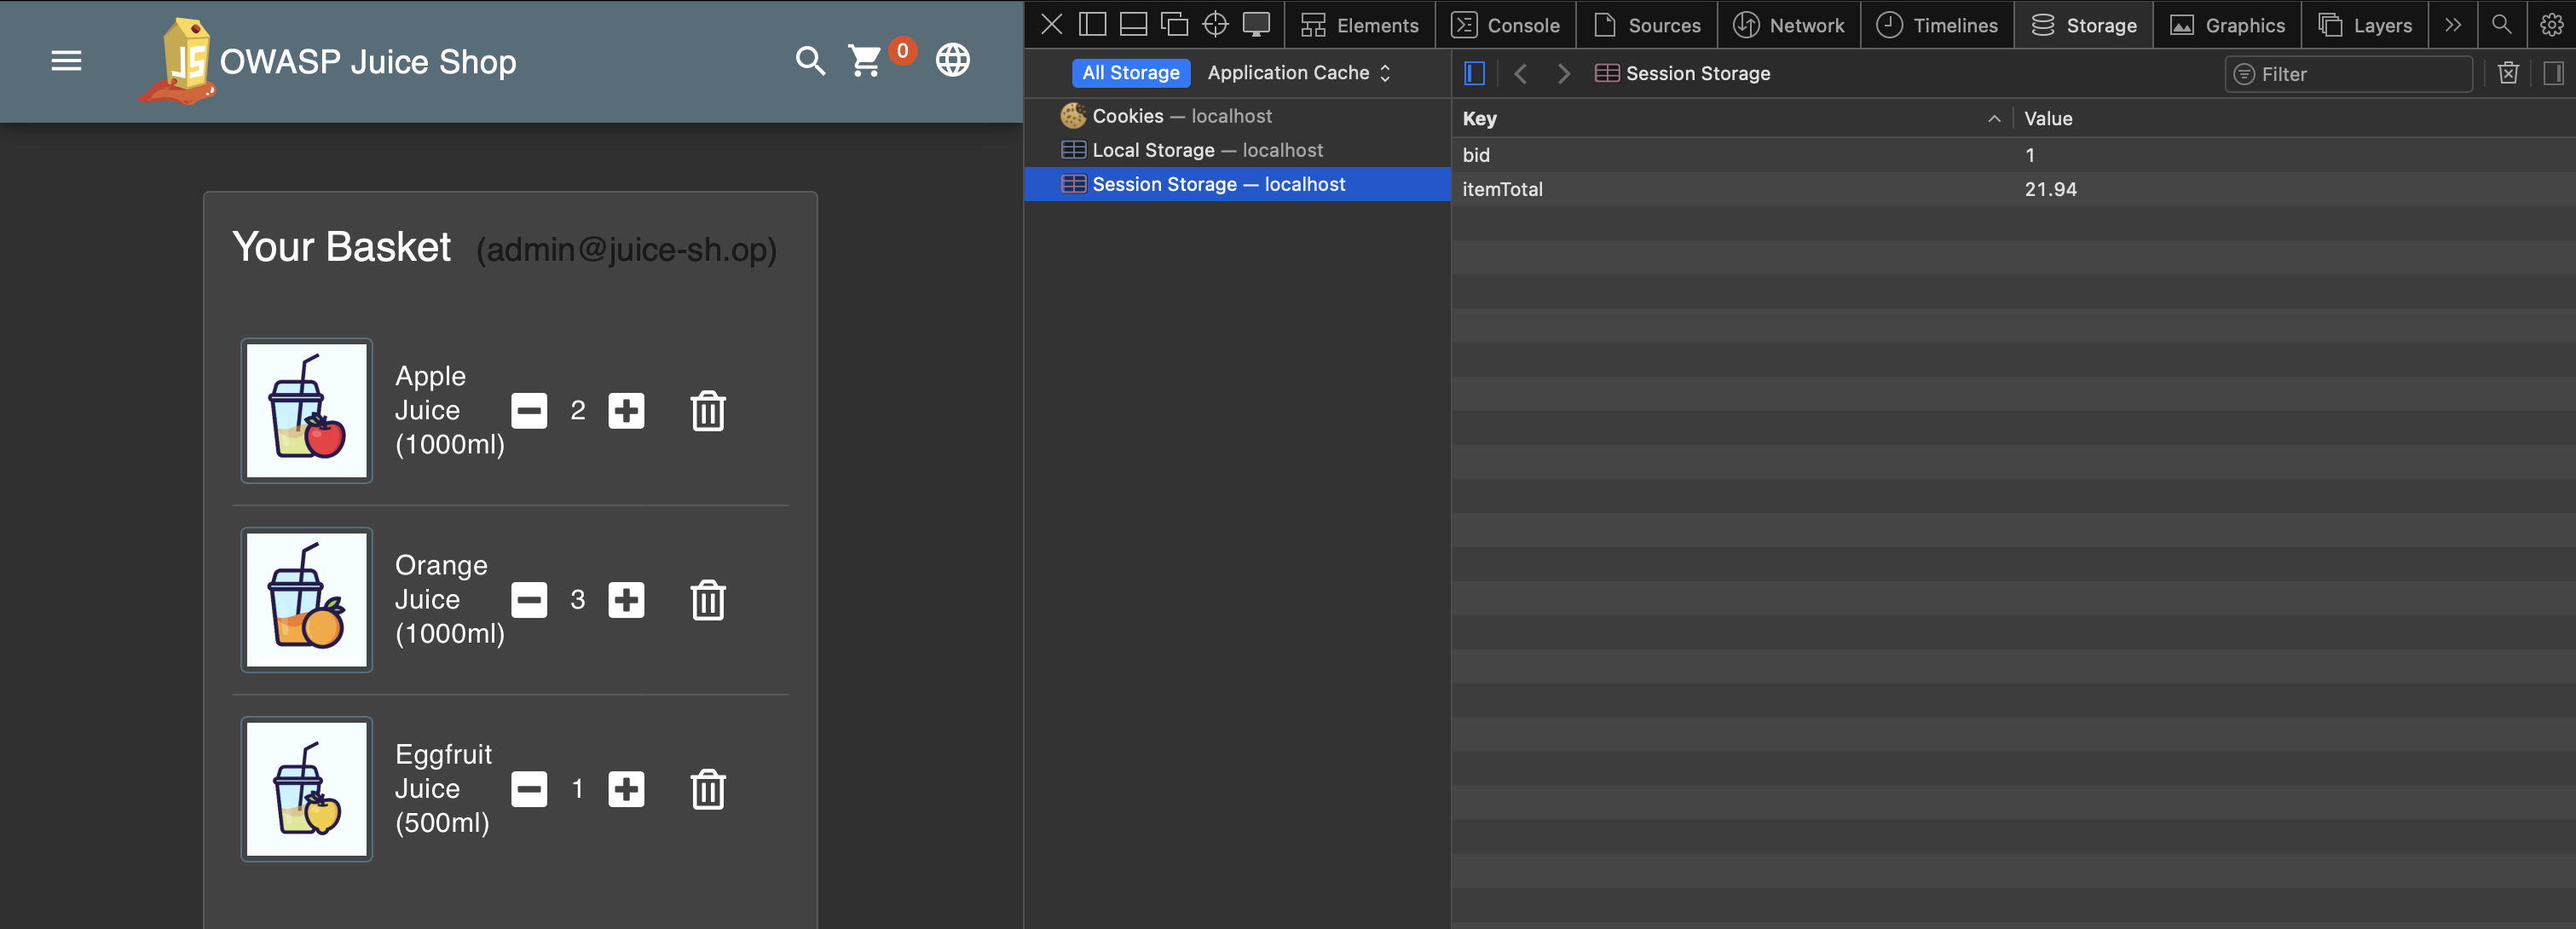
\includegraphics[width=.9\textwidth]{q1}
\end{center}

Сейчас мы в своей корзине, через локальное хранилище можно увидеть где хранится id корзины.
Попробуем его поменять на id корзины другого пользователя.

\begin{center}
  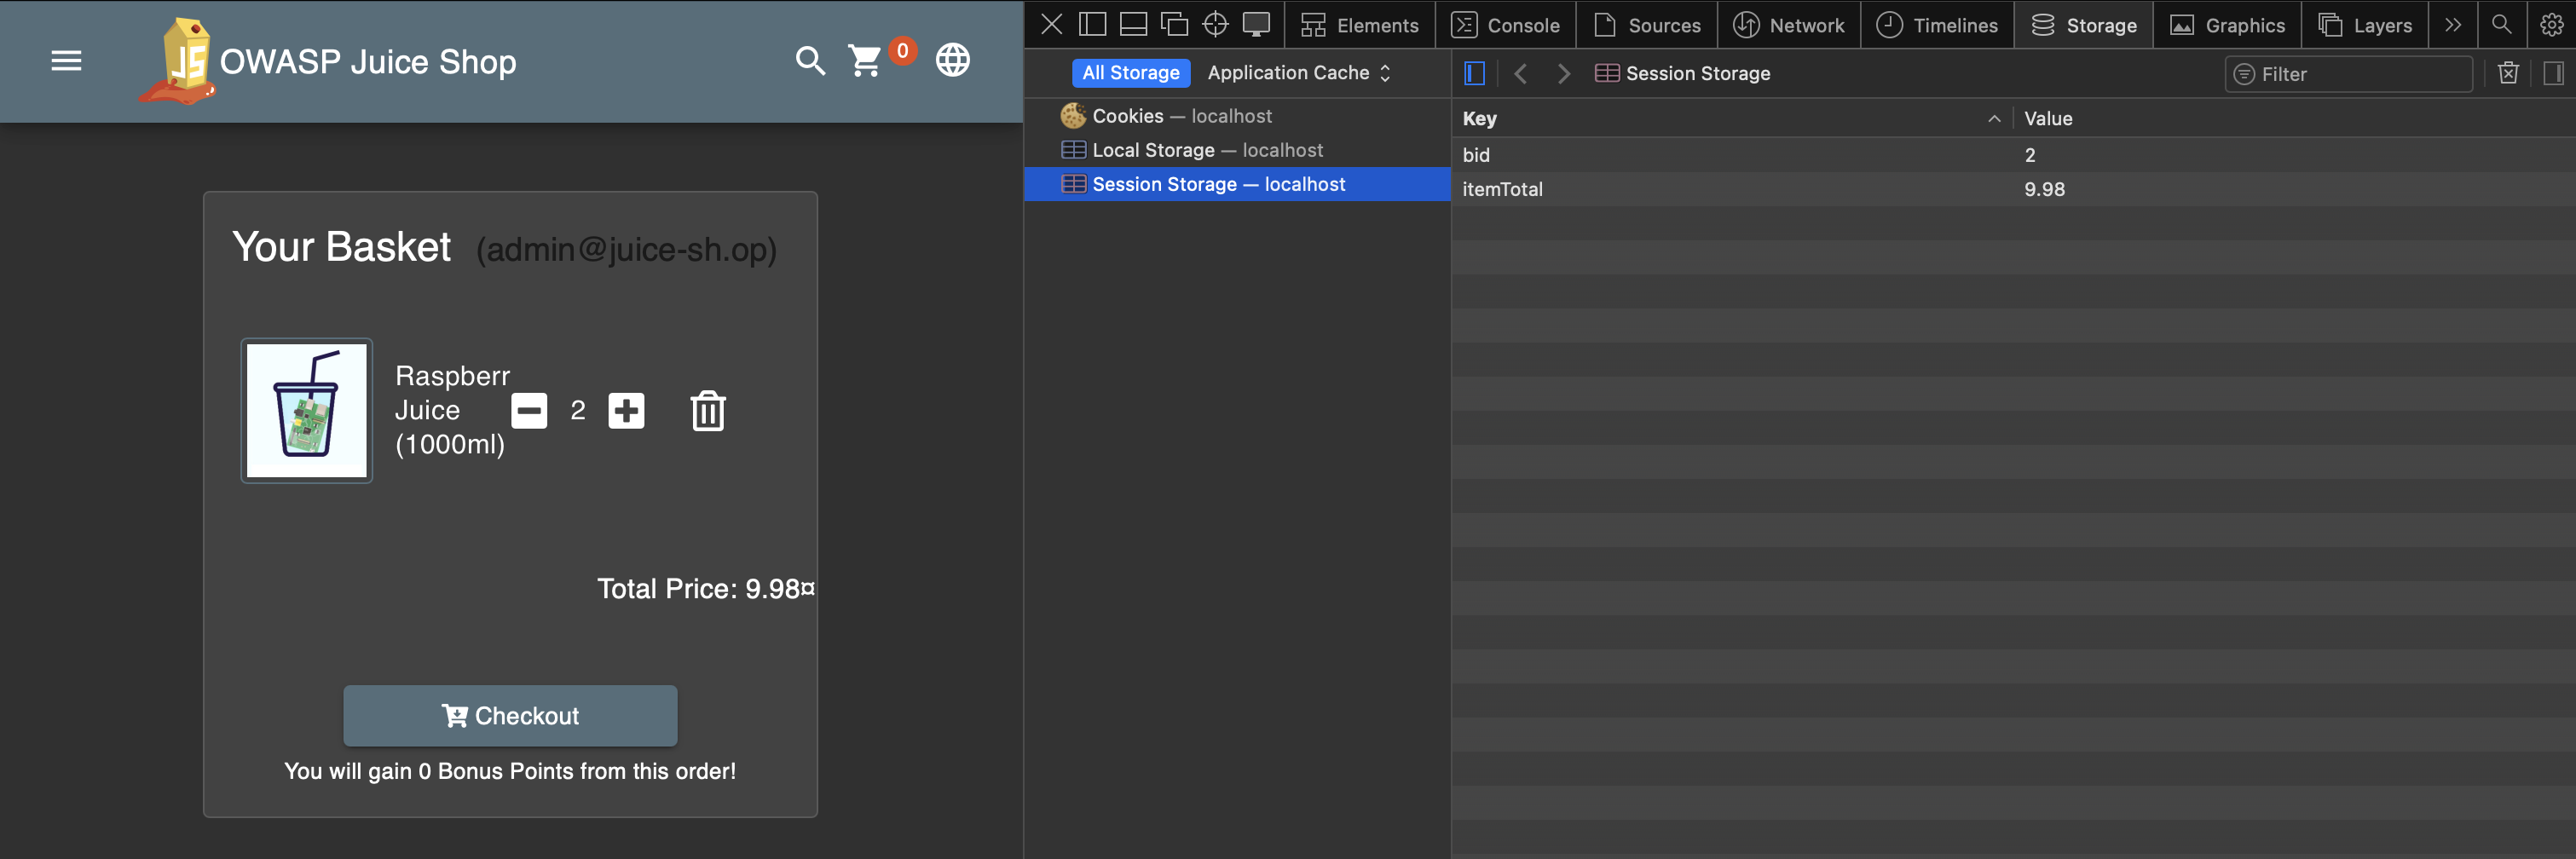
\includegraphics[width=.9\textwidth]{q11}
\end{center}

Мы успешно получили доступ к чужой корзине и можем её редактировать и далее вернуться в свою корзину.

\subsection{Broken Access Control}

Попробуем оставить фидбэк от не своего имени, так как возможно, что логин отправителя фидбэка будет вычислен не на сервере, а на клиенте.

На данный момент видно, что поле с вводом логина для фидбэка отключено для ввода и там по умолчанию наш логин.

\begin{center}
  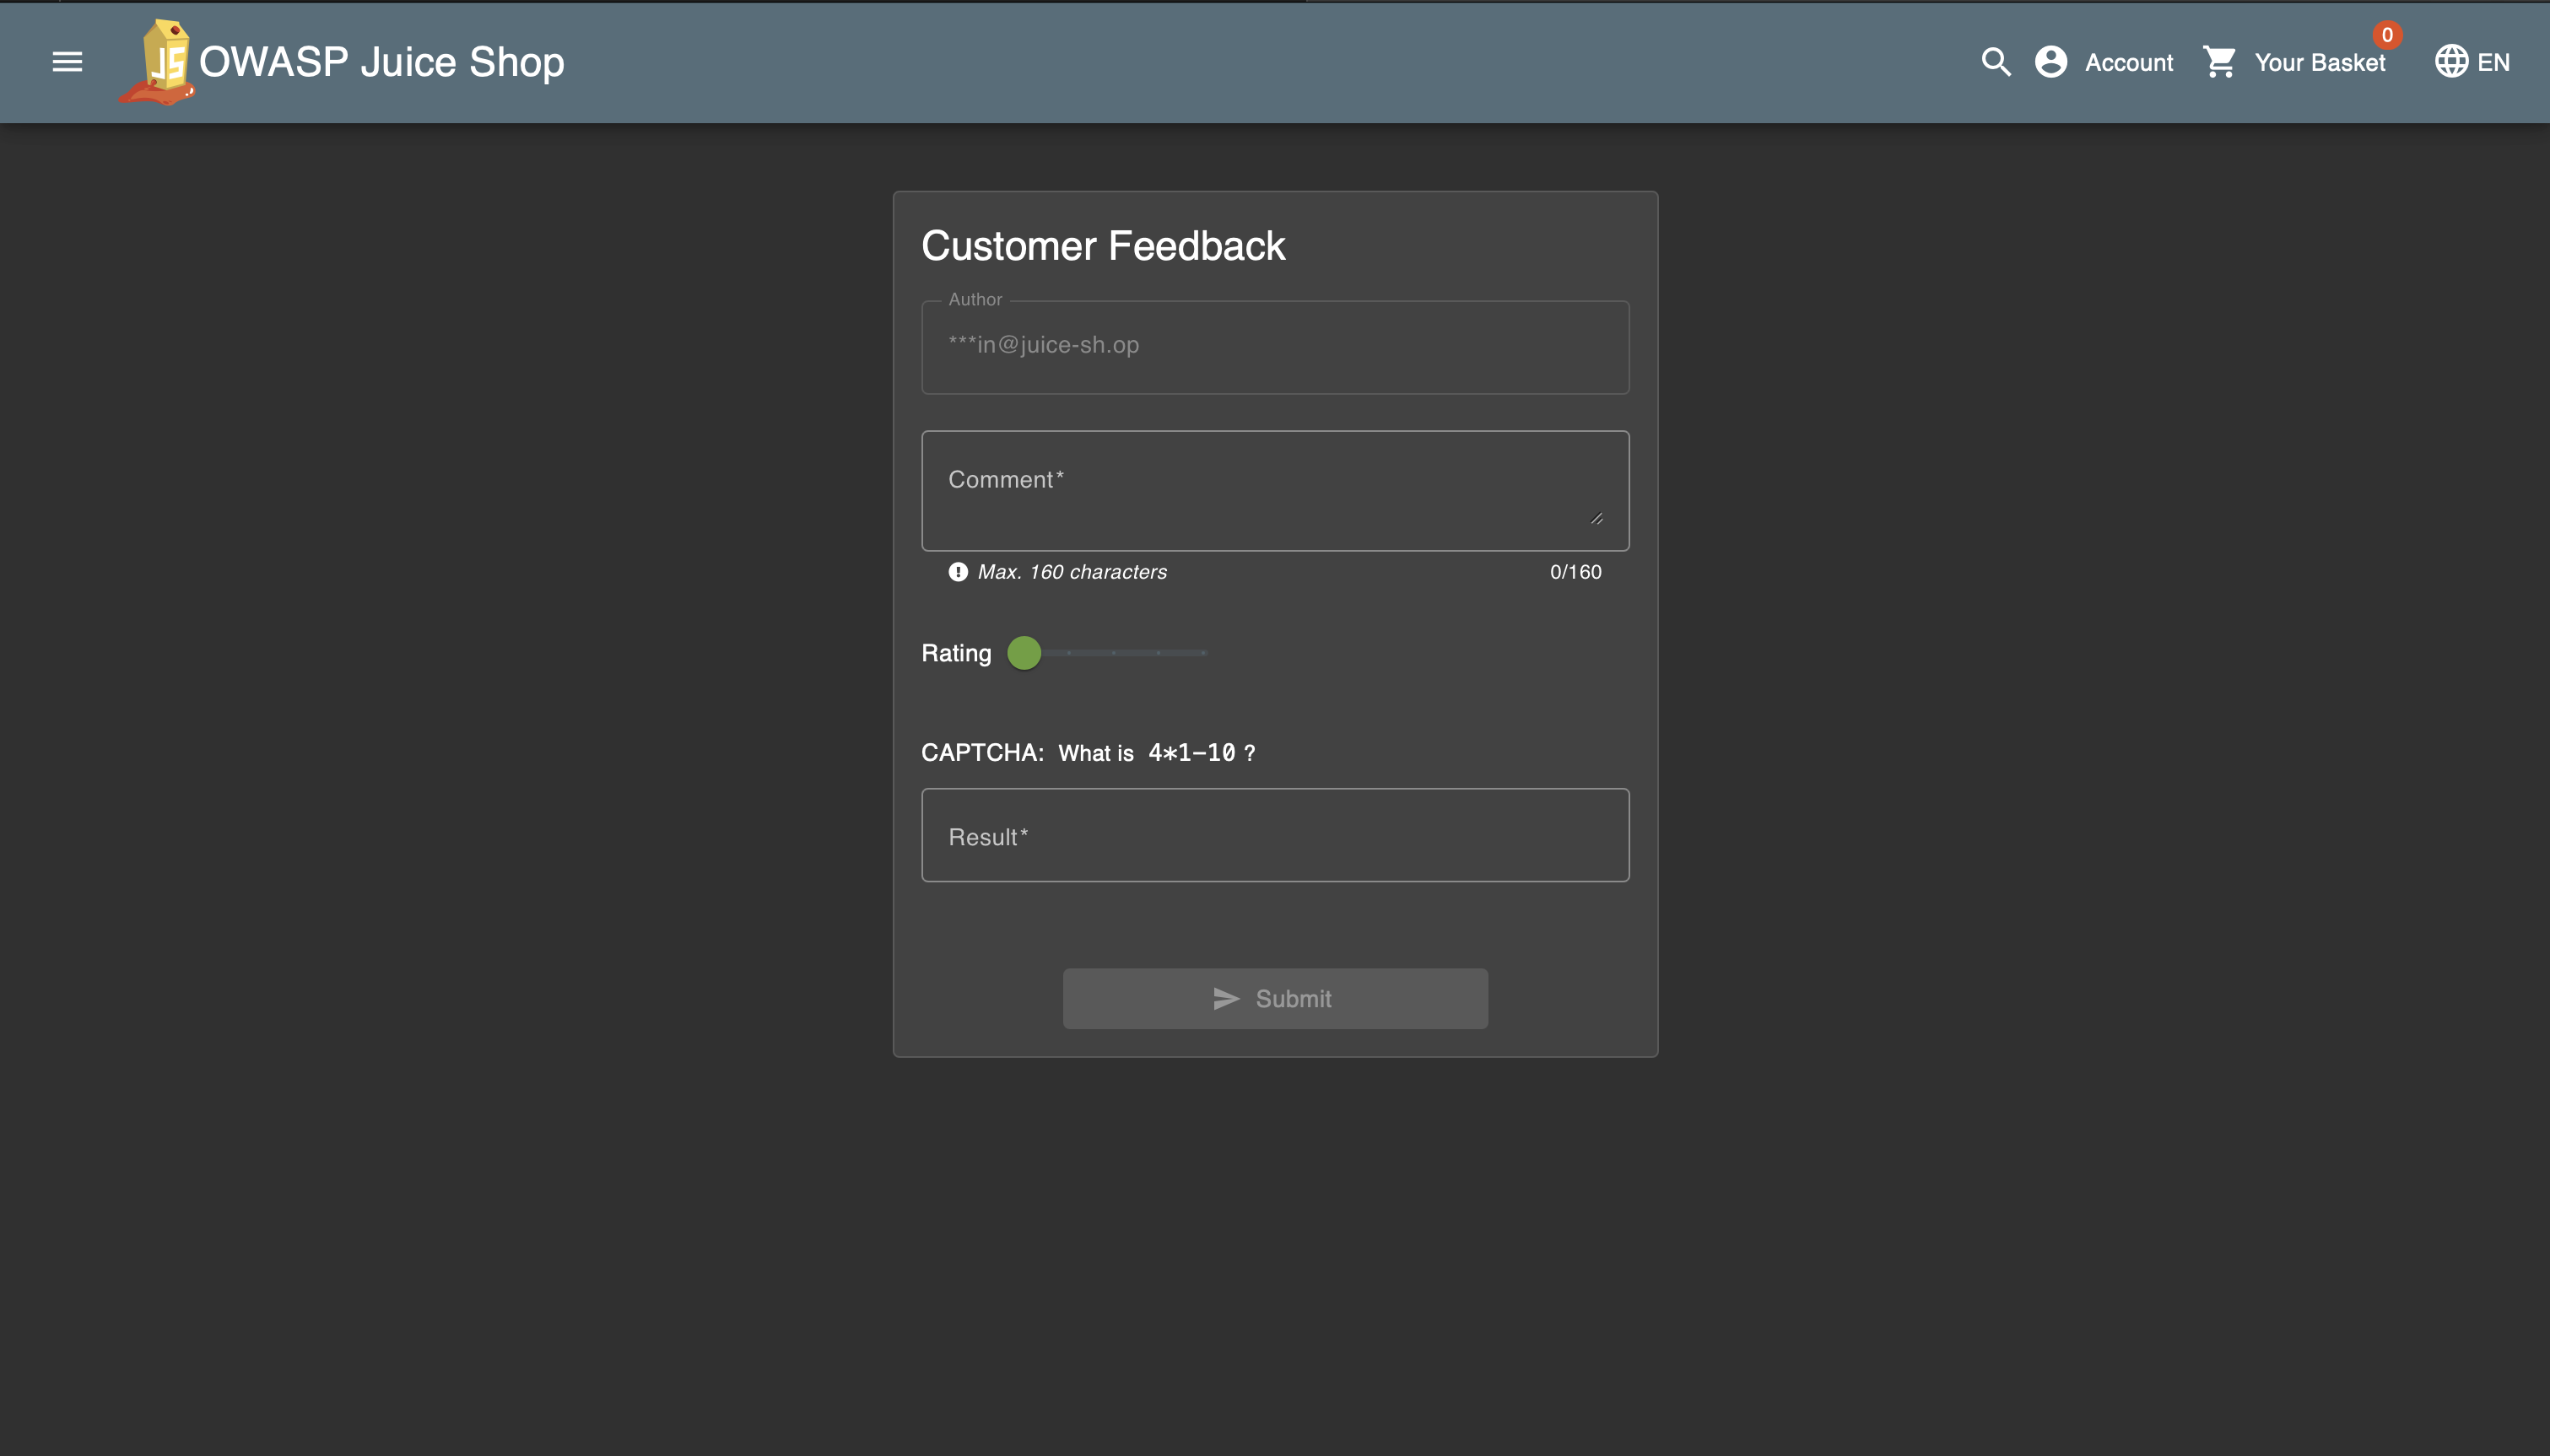
\includegraphics[width=.9\textwidth]{s1}
\end{center}

Попробуем ввести фидбэк от имени другого пользователя и для этого поменяем через dev tools дефолтный логин. 
Достаточно было отключить disable атрибут у input с логином и ввести другой логин.

\begin{center}
  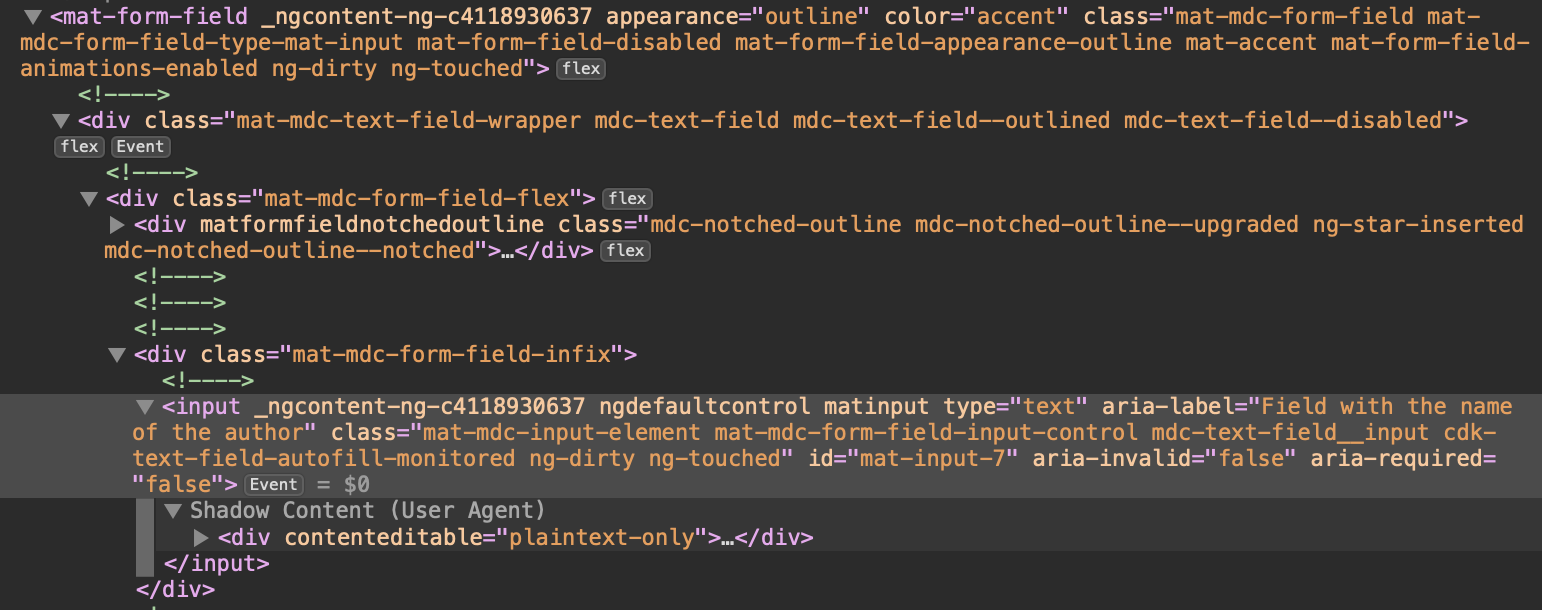
\includegraphics[width=.9\textwidth]{s11}
\end{center}

Отправка фидбэка прошла успешно.

\begin{center}
  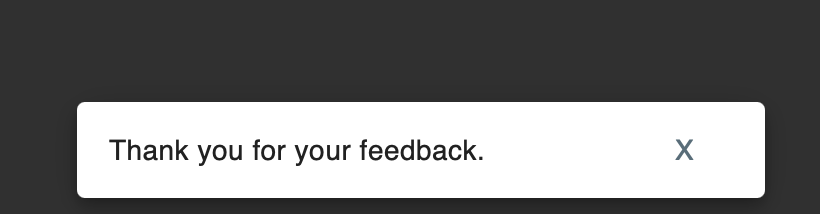
\includegraphics[width=.9\textwidth]{s111}
\end{center}

Мы отправили фидбэк от имени другого пользователя (anonimous). Вот ответ от сервера, что он сохранил в базу данных.

\begin{center}
  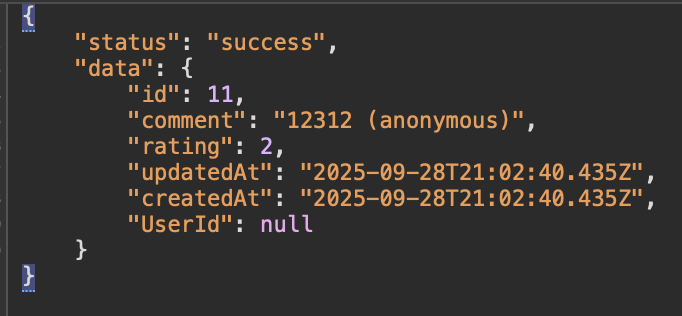
\includegraphics[width=.9\textwidth]{s1111}
\end{center}

\section{Data Flow Diagram — DFD}

\subsection{Диаграмма}

\begin{center}
  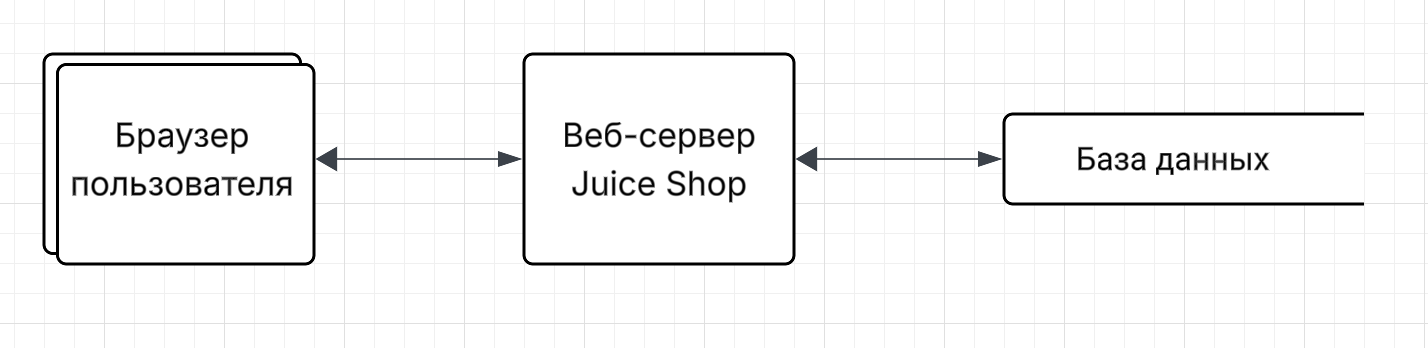
\includegraphics[width=.9\textwidth]{dfd}
\end{center}

\subsection{Потоки данных}

\begin{center}
  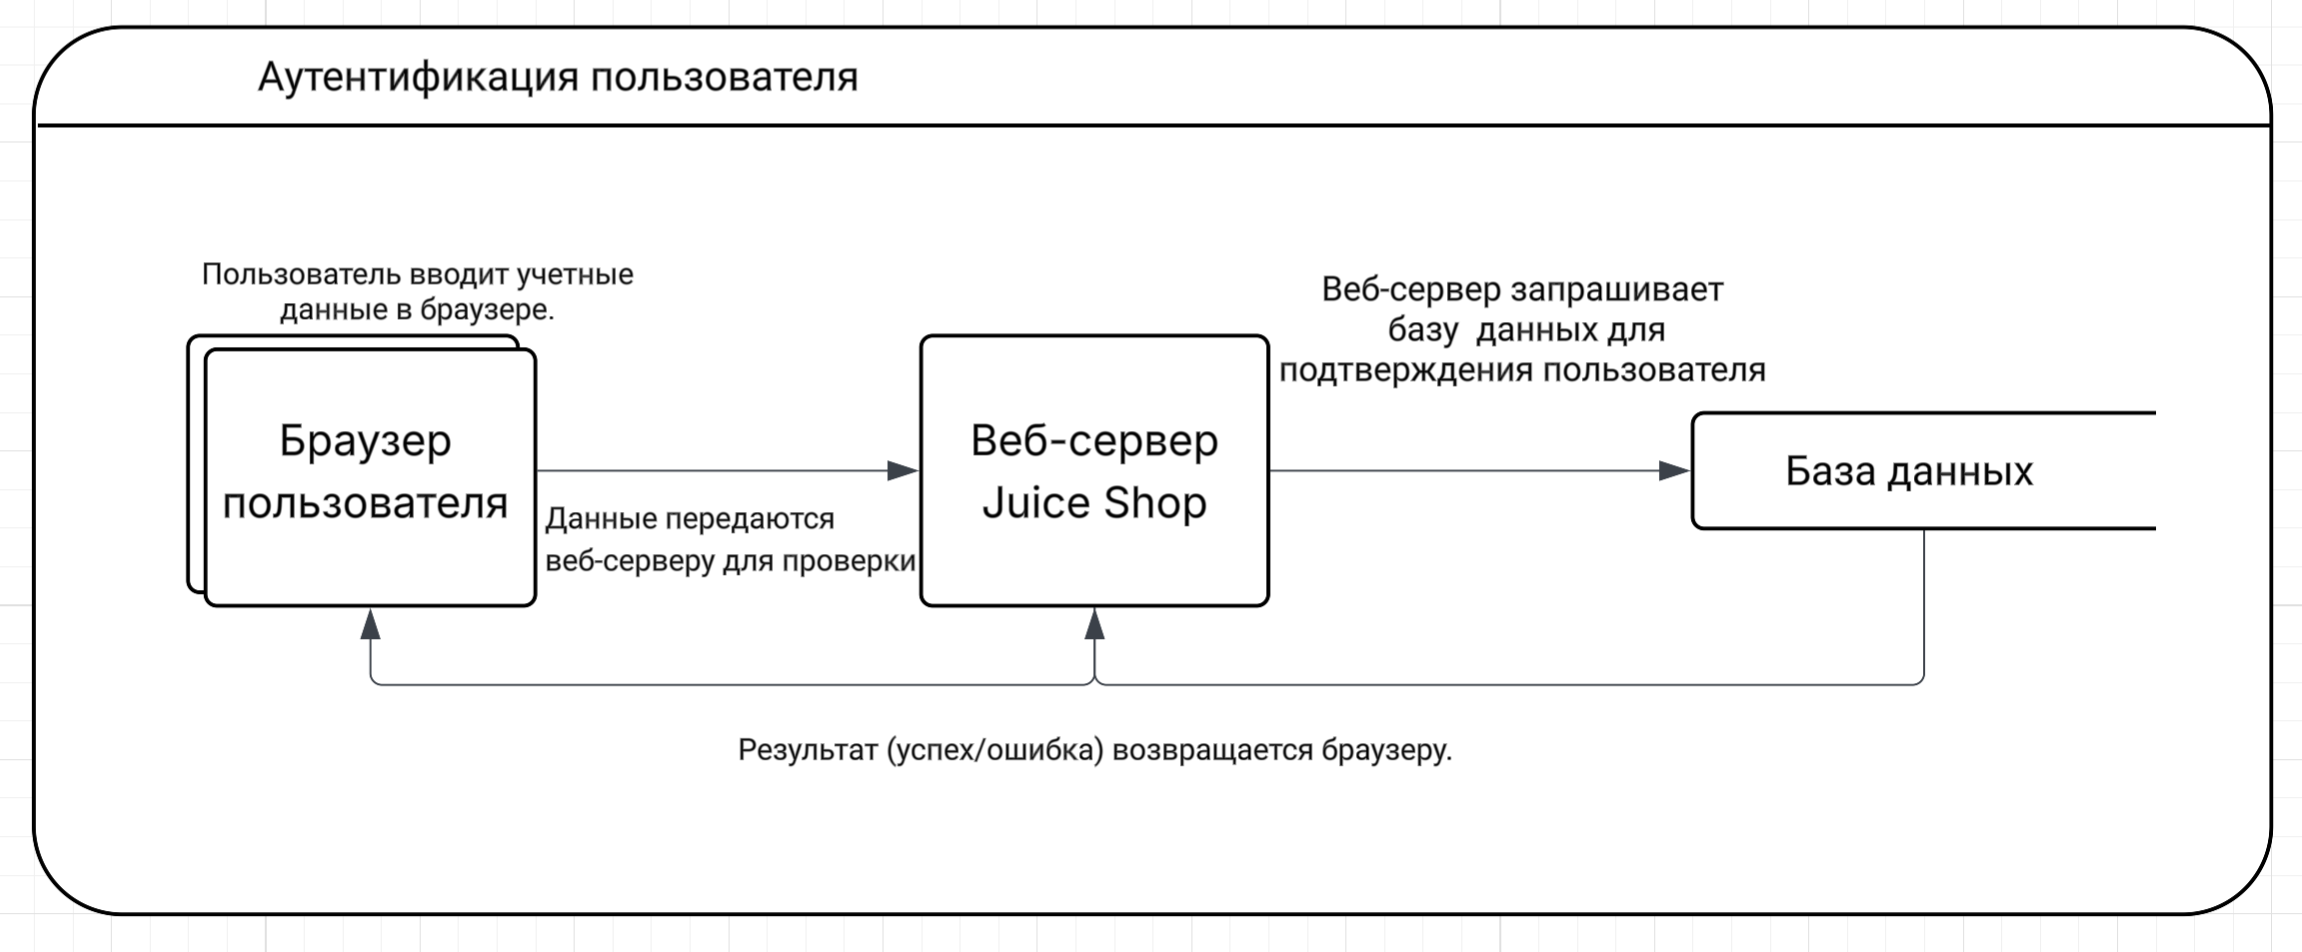
\includegraphics[width=.9\textwidth]{auth}
\end{center}

\begin{center}
  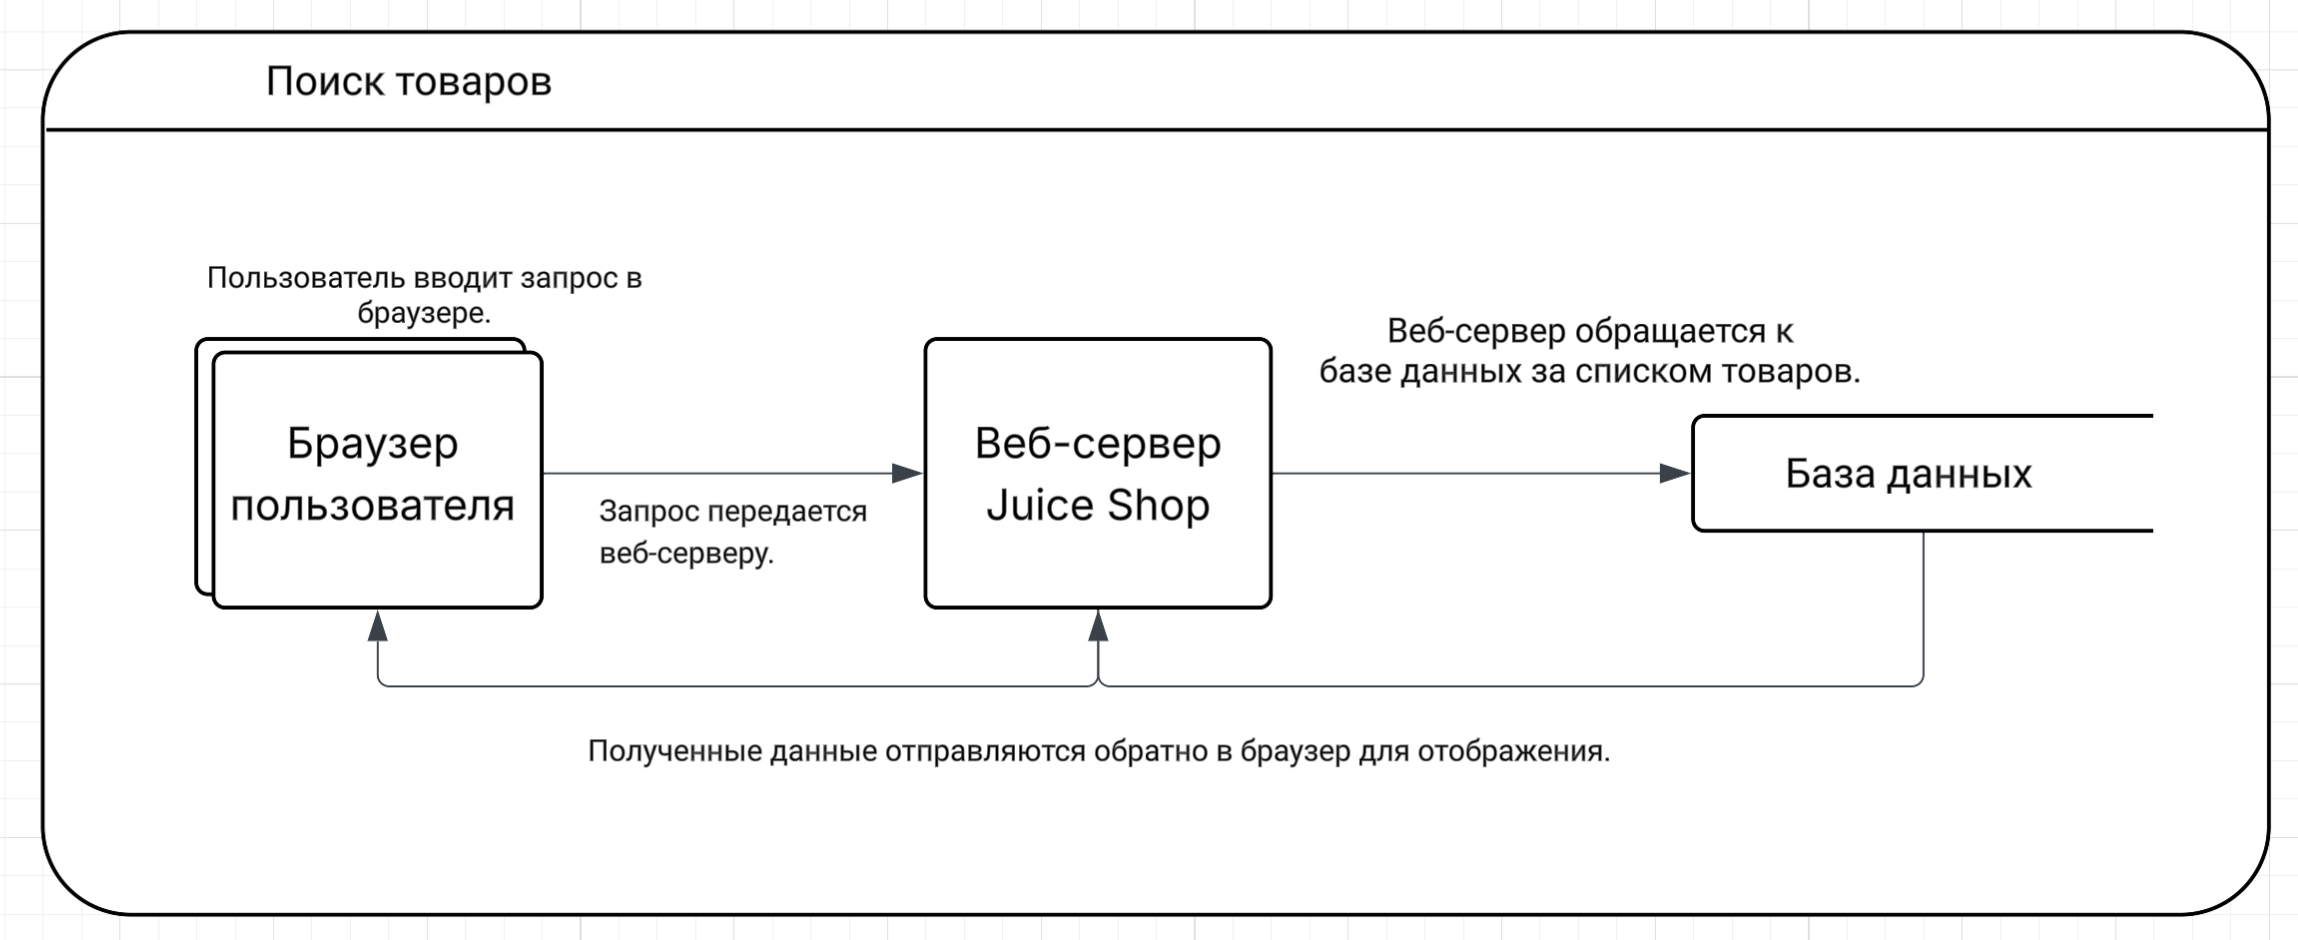
\includegraphics[width=.9\textwidth]{sear}
\end{center}

\begin{center}
  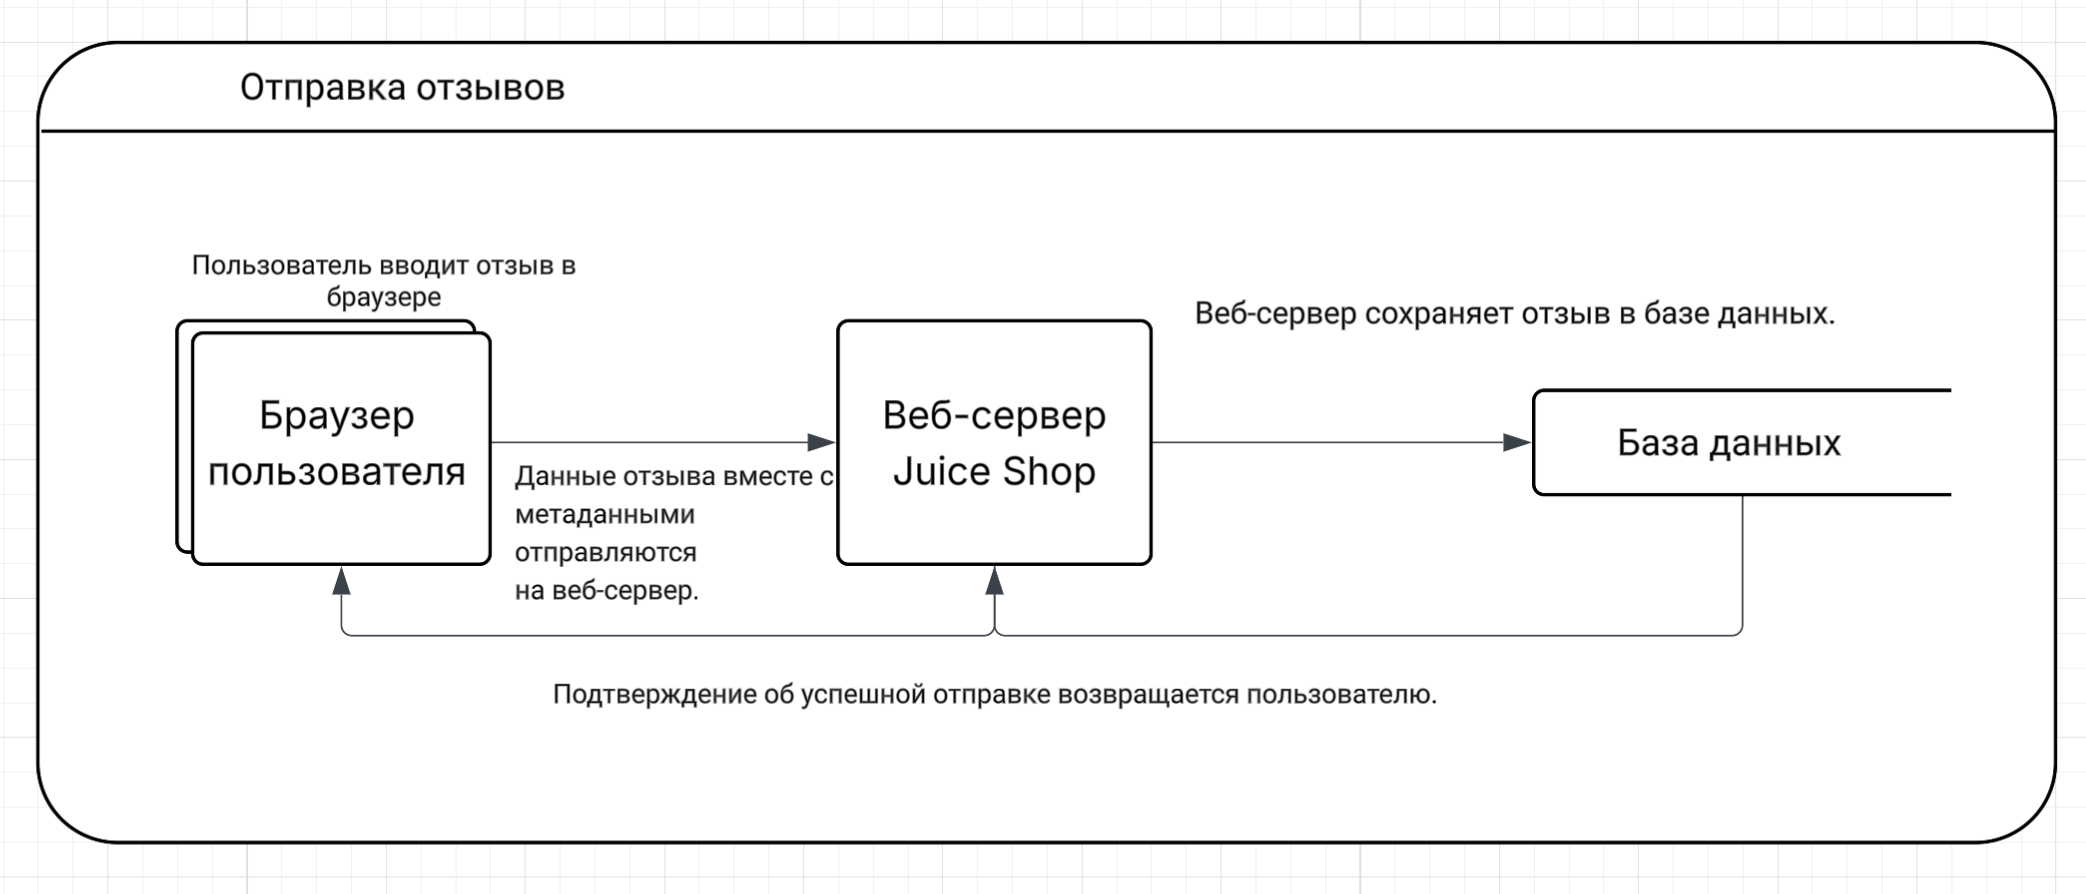
\includegraphics[width=.9\textwidth]{fee}
\end{center}

\begin{center}
  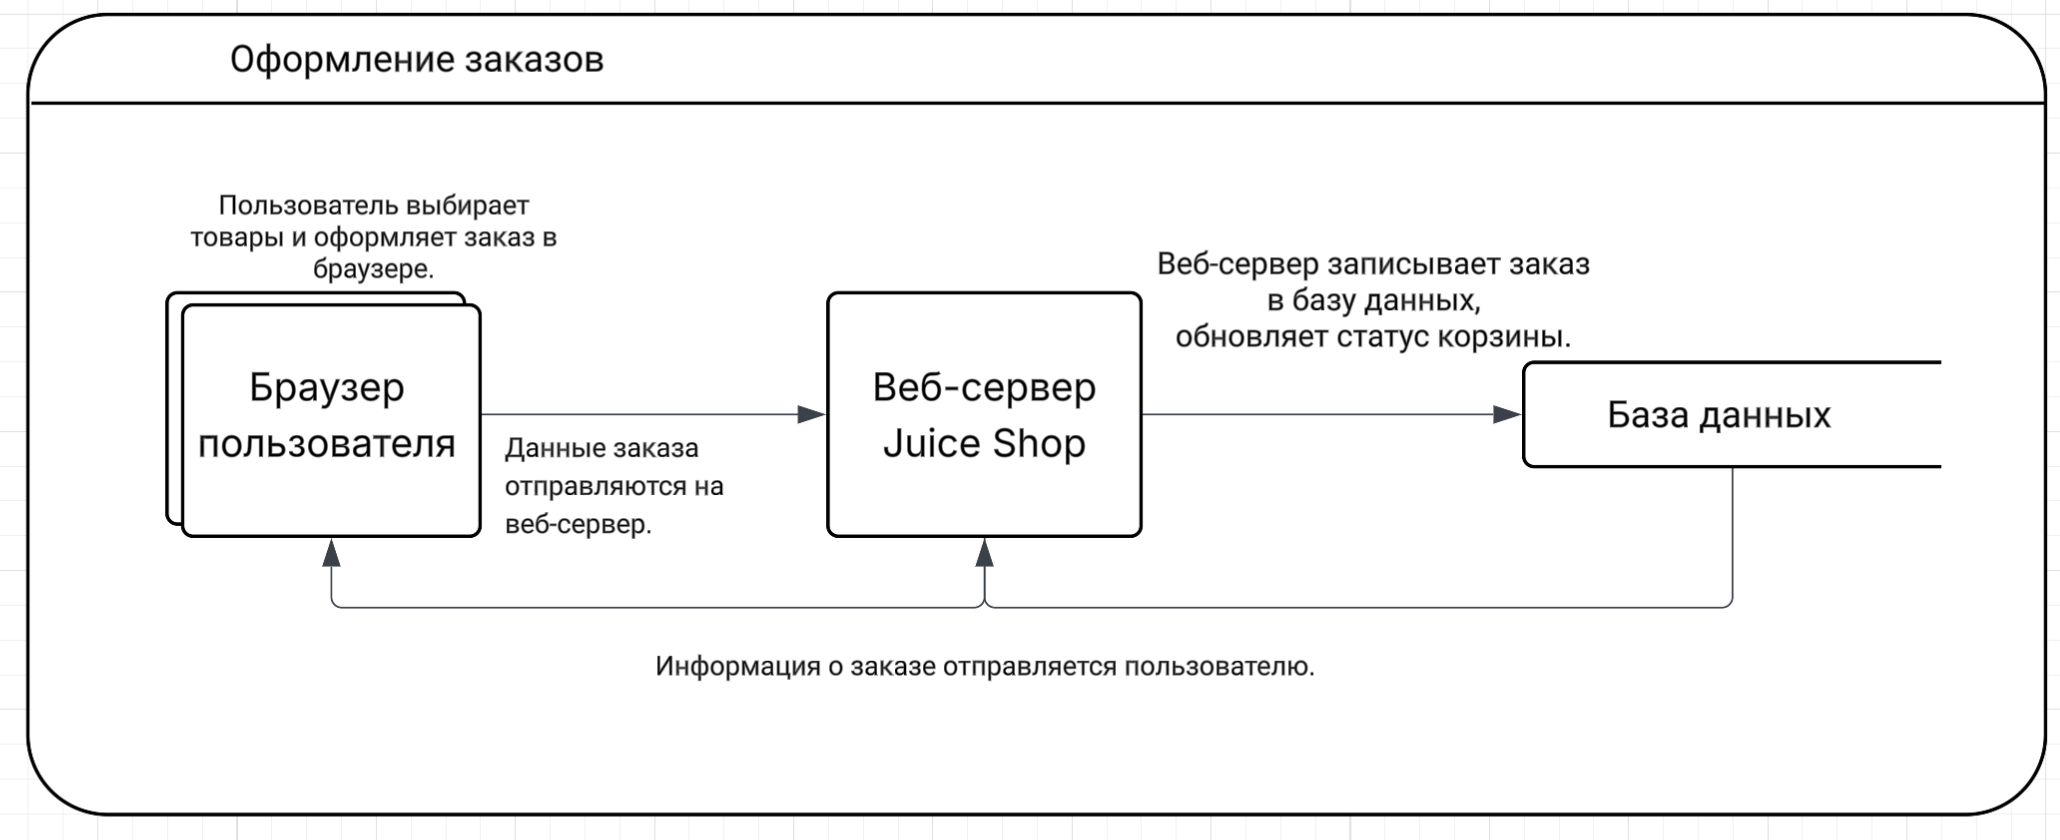
\includegraphics[width=.9\textwidth]{ord}
\end{center}


\section{Анализ угроз по методике STRIDE}

\subsection{Spoofing (Маскировка)}

\begin{itemize}
    \item \textbf{SQL Injection в аутентификации} - возможность входа под любым пользователем через SQL-инъекцию \texttt{OR 1=1--}
    \item \textbf{Подмена отправителя фидбэка} - возможность отправки фидбэка от имени другого пользователя через изменение параметров в DevTools
\end{itemize}

\textbf{Описание:} SQL-инъекция позволяет обойти аутентификацию и войти в систему под любым пользователем, включая администратора. Изменение параметров фидбэка через DevTools позволяет отправлять сообщения от имени других пользователей.

\subsection{Tampering (Изменение данных)}

\begin{itemize}
    \item \textbf{Доступ к чужим корзинам} - возможность изменения содержимого корзины другого пользователя через изменение ID в localStorage
    \item \textbf{Подмена отправителя фидбэка} - возможность изменения автора фидбэка
\end{itemize}

\textbf{Описание:} Через изменение ID корзины в localStorage можно получить доступ к корзине другого пользователя и изменять её содержимое. Также можно изменять автора фидбэка, что приводит к искажению данных в системе.

\subsection{Repudiation (Отказ от операций)}

\begin{itemize}
    \item \textbf{Отсутствие логирования действий} - нет возможности отследить, кто именно совершил действия в системе
    \item \textbf{Подмена отправителя фидбэка} - пользователь может отрицать отправку фидбэка, так как система не проверяет подлинность отправителя
\end{itemize}

\textbf{Описание:} Из-за отсутствия надлежащего логирования и проверки подлинности пользователей, невозможно доказать, кто именно совершил определенные действия в системе.

\subsection{Information Disclosure (Раскрытие информации)}

\begin{itemize}
    \item \textbf{Учетные данные в исходном коде} - логин и пароль администратора хранятся в открытом виде в файле main.js
    \item \textbf{SQL Injection} - возможность получения доступа к данным всех пользователей через SQL-инъекции
    \item \textbf{Доступ к чужим корзинам} - возможность просмотра содержимого корзины других пользователей
\end{itemize}

\textbf{Описание:} Критические учетные данные администратора находятся в исходном коде приложения, что позволяет любому пользователю получить полный доступ к системе. SQL-инъекции позволяют извлекать данные из базы данных.

\subsection{Denial of Service (Отказ в обслуживании)}

\begin{itemize}
    \item \textbf{XSS атаки} - выполнение произвольного JavaScript кода может привести к нестабильной работе приложения
    \item \textbf{SQL Injection} - некорректные SQL-запросы могут привести к перегрузке базы данных
\end{itemize}

\textbf{Описание:} XSS атаки могут нарушить работу пользовательского интерфейса, а SQL-инъекции могут вызвать перегрузку базы данных, что приведет к отказу в обслуживании.

\subsection{Elevation of Privilege (Повышение привилегий)}

\begin{itemize}
    \item \textbf{SQL Injection в аутентификации} - получение прав администратора через SQL-инъекцию
    \item \textbf{Использование учетных данных из исходного кода} - вход под тестовым аккаунтом с найденными в коде учетными данными
\end{itemize}

\textbf{Описание:} SQL-инъекция позволяет обойти систему аутентификации и получить права администратора. Также учетные данные администратора в исходном коде позволяют любому пользователю получить полные права в системе.

\section{Таблица уязвимостей}

Калькулятор уровня риска использовал \href{https://bdu.fstec.ru/calc3}{https://bdu.fstec.ru/calc3}

\begin{table}[h!]
\centering
\small
\begin{tabular}{|p{2.5cm}|p{3.5cm}|p{1.5cm}|p{2cm}|p{3.5cm}|}
\hline
\textbf{Название} & \textbf{Описание} & \textbf{Уровень риска (CVSS)} & \textbf{OWASP Top 10} & \textbf{Предложение по исправлению} \\
\hline
SQL Injection в аутентификации & Возможность обхода аутентификации через SQL-инъекцию \texttt{OR 1=1--} в поле логина. Позволяет войти под любым пользователем, включая администратора. & 9.8 (Critical) & A03:2021 - Injection & Использовать параметризованные запросы, валидировать и экранировать пользовательский ввод на сервере \\
\hline
Stored XSS в поиске & Возможность внедрения произвольного JavaScript кода через поле поиска. Код сохраняется и выполняется для всех пользователей. & 8.8 (High) & A03:2021 - Injection & Валидировать и экранировать пользовательский ввод, внедрить Content Security Policy (CSP) \\
\hline
Sensitive Data Exposure & Учетные данные (логин и пароль) хранятся в открытом виде в файле main.js & 7.5 (High) & A02:2021 - Cryptographic Failures & Удалить учетные данные из исходного кода, использовать переменные окружения, внедрить безопасное хранение паролей \\
\hline
Broken Access Control - корзины & Возможность доступа к корзине другого пользователя через изменение ID в localStorage & 6.5 (Medium) & A01:2021 - Broken Access Control & Проверять права доступа на сервере, не полагаться на клиентские данные для авторизации \\
\hline
Broken Access Control - фидбэк & Возможность отправки фидбэка от имени другого пользователя через изменение параметров в DevTools & 5.3 (Medium) & A01:2021 - Broken Access Control & Проверять подлинность пользователя на сервере, использовать серверные сессии \\
\hline
\end{tabular}
\caption{Таблица найденных уязвимостей}
\end{table}

\section{Рекомендации по устранению рисков}

\begin{enumerate}
    \item \textbf{Внедрить строгую валидацию данных:} Все пользовательские данные должны валидироваться и экранироваться на стороне сервера. Использовать параметризованные запросы для предотвращения SQL-инъекций.
    
    \item \textbf{Реализовать Content Security Policy (CSP):} Ограничить выполнение JavaScript кода только из доверенных источников.
    
    \item \textbf{Усилить систему аутентификации и авторизации:} Удалить учетные данные из исходного кода, реализовать проверку прав доступа на сервере для всех операций.
    
    \item \textbf{Внедрить логирование и мониторинг:} Реализовать детальное логирование всех действий пользователей для обеспечения возможности аудита и обнаружения подозрительной активности. Добавить триггеры для отправки уведомлений на email администратора об странных дейсвиях.
    
    \item \textbf{Регулярно обновлять зависимости:} Внедрить процесс регулярного обновления всех используемых библиотек для устранения известных уязвимостей.
    \item 
    \item \textbf{Доработка пайплайнов:} Внедрить в пайпланы статические, динамические проверки на уязвимости.
\end{enumerate}

\section*{Вывод}

Освоил методику комплексного анализа защищенности веб-приложения, сочетая
автоматизированное сканирование (DAST) и проактивное моделирование угроз (Threat Modeling).
Получил навыки документирования результатов аудита в виде профессионального отчета.

\end{document}

\begin{center}
  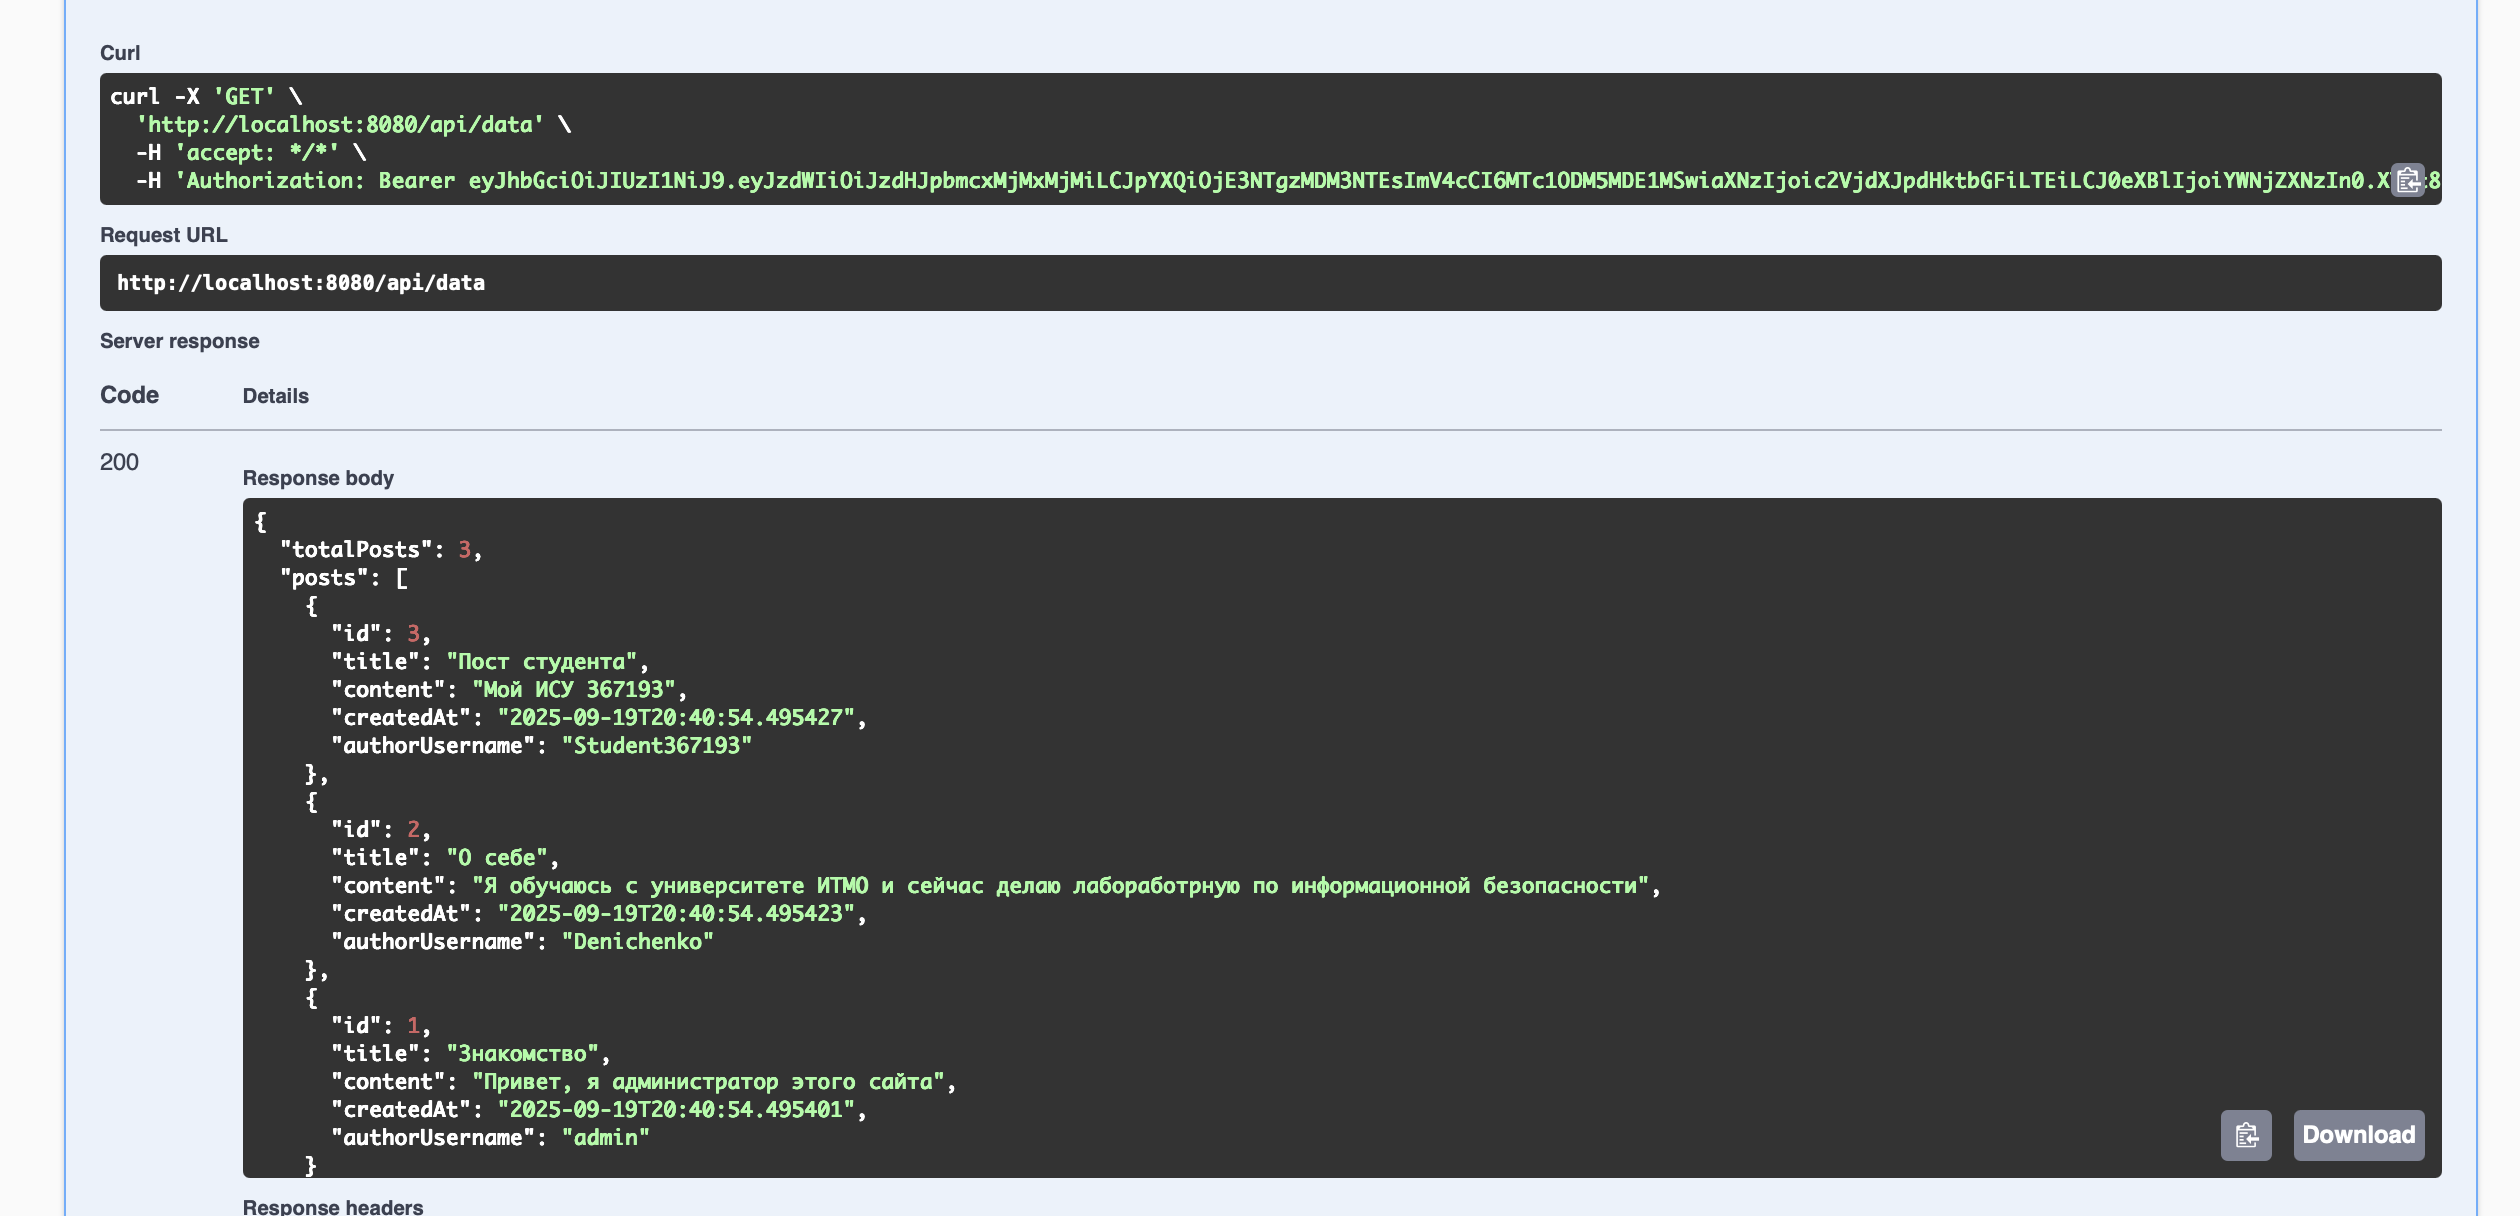
\includegraphics[width=.9\textwidth]{posts}
\end{center}

\href{https://github.com/Alex-de-bug/security-lab-1/actions/runs/17864752066}{Последний верный CI} (https://github.com/Alex-de-bug/security-lab-1/actions/runs/17864752066)
http://testaspnet.vulnweb.com